\documentclass[11pt,a4paper]{article}
\usepackage[margin=2.2cm]{geometry}
\usepackage{parskip}
\setlength{\parskip}{4pt}
\usepackage[T1]{fontenc}
\usepackage[utf8]{inputenc}
\usepackage{mathptmx}   % Times for text AND math, so digits and symbols match the body font
\usepackage{textcomp}
\usepackage{microtype}
\usepackage{amsmath,amssymb,amsfonts}
\usepackage{graphicx}
\usepackage{xcolor}
\usepackage{booktabs}
\usepackage{multirow}
\usepackage{tabularx}
\usepackage{array}
\usepackage{url}
\usepackage{cite}
\usepackage{pifont}
\usepackage{tikz}
\usetikzlibrary{shapes.geometric, arrows.meta, positioning, fit, calc}
\usepackage{pgfplots}
\pgfplotsset{compat=1.18}
\usepackage{caption}
\usepackage{subcaption}
\usepackage{placeins}
\usepackage[hidelinks]{hyperref}
\urlstyle{same}

\captionsetup{font=footnotesize,labelfont=bf}
\captionsetup[subfigure]{labelfont=rm,textfont=rm}
\setlength{\textfloatsep}{7pt plus 2pt minus 2pt}
\setlength{\floatsep}{7pt plus 2pt minus 2pt}
\setlength{\intextsep}{7pt plus 2pt minus 2pt}
\setlength{\abovecaptionskip}{3pt}
\setlength{\belowcaptionskip}{0pt}
\newcommand{\cmark}{\ding{51}}
\newcommand{\xmark}{\ding{55}}
% typography: bold only marks the best value in a table column; italics only for run-in headings and a term's first definition
\newenvironment{IEEEkeywords}{\par\smallskip\noindent\textit{Keywords---}}{\par}
\newcommand{\runin}[1]{\textit{#1}}
\newcommand{\vfour}{v4}

\begin{document}

\title{\textbf{AsanaAI: Project Report}\\[4pt]
\large Design, Implementation, Deployment and Verification of a Privacy-Preserving\\
Yoga Posture Coach on Commodity Hardware}
\author{Anamitra Sarkar \and Debjit Deb Barman \and Adrija Ray Mondal \and Tanima Samanta\\[6pt]
Supervisor: Mr.\ Sujit Chakraborty, Assistant Professor, Dept.\ of CSE (AI/ML)\\[2pt]
RCC Institute of Information Technology, Kolkata, West Bengal, India}
\date{}

\maketitle
\tableofcontents
\clearpage

\begin{abstract}
Practising yoga without an instructor can risk injury, yet automated coaches are usually validated on random train/validation splits that overstate how well they work for new people, rooms and cameras.
We present AsanaAI, a browser-based yoga posture coach in which the camera image never leaves the device: the page extracts 33 body landmarks, and only those numbers reach a small CPU server.
The server runs a cascade of 3-head residual MLPs (one model names the pose, a second vetoes photos that are not one of the app's poses and scores form), a rule engine that turns joint-angle bands into per-joint cues, and an ST-GCN over the 33-joint skeleton as a second opinion on held poses.
Training labels come from 24 instructor-led videos (1.2\,M frames) and are cue-verified: the instructor names the pose in a Whisper transcript, a biomechanical rule engine agrees, and the pose is held steady.
Scoring only on data never used in training, the cascade names the pose on 78.9\% of 1{,}685 held-out public photos with a 20.8\% false-alarm rate on photos of other poses and clears a 0.70 recall/precision bar on seven poses; the rules-only path it replaces reaches 36.9\%, 78.3\% and none.
On held-out videos the ST-GCN reaches 78.0\% macro recall, against 19--21\% for the sequence model it replaces.
Against standard methods trained on the same data, a random forest is stronger on held-out photos from the training sources (85.3\% vs.\ 78.9\% overall) but weakest on wild photos from another source (35.0\% vs.\ 55.3\%), so no single method wins everywhere.
Deployment work makes this usable on budget phones: a pose-engine fallback ladder for a GPU driver that crashes MediaPipe, visibility-aware scoring that declines to judge joints the camera cannot see, a personal range-of-motion calibration, an on-device port of the rule engine (0 mismatches over 12{,}500 parity cases), and English/Hindi/Bengali coaching passed through a safety screen.
We report what does not work: no live-person accuracy study yet, weak mountain, cobra and child's pose, and a form score that is nearly blind to arm errors.
\end{abstract}

\begin{IEEEkeywords}
yoga posture correction, pose estimation, residual MLP, ST-GCN, occlusion, on-device inference, held-out evaluation
\end{IEEEkeywords}


\section{Introduction}
Yoga is practised worldwide---the United Nations proclaimed an International Day of Yoga in 2014 \cite{unga2014yoga}---and it is increasingly learned alone, from videos and phone apps, with nobody to correct the posture. A systematic review of published case reports and case series documented adverse events associated with yoga \cite{cramer2013yoga}. A camera-based coach that tells a practitioner which joint is off, in their own language and without frightening or pushing them, is therefore attractive. Real-time body-landmark estimators that run on a phone \cite{bazarevsky2020blazepose,lugaresi2019mediapipe} make it technically possible; making it trustworthy on ordinary hardware is harder, and this paper is about that gap.

We build on three observations from developing and testing AsanaAI.

\runin{(1) Random-split accuracy is not accuracy.} Video frames and web photos have near-duplicate neighbours, mirrored copies and repeated photographs; when these fall on both sides of a random split, validation accuracy measures memory, a form of leakage known to inflate reported results across many fields \cite{kapoor2023leakage}. The first model of this project reached 91.5\% on its random validation split; on held-out photos it passed none of the poses and raised a false alarm on 75\% of photos of poses outside its vocabulary (Section~\ref{sec:results}). We therefore report only numbers measured on data a model never trained on.

\runin{(2) A coach must be deployable where its users are.} Phones differ widely in their GPU drivers. On one budget phone (MediaTek Dimensity 7025, PowerVR BXM-8-256 GPU) we found that the standard MediaPipe web engine aborts inside the driver, and we chose to send no image to a server, because a camera pointed at a person at home should not become an upload.

\runin{(3) Feedback has to be honest about what is not seen.} A pose estimator happily invents joints that are hidden; a coach that scores an invented knee is worse than silent. And a generated sentence must never tell someone to push through pain.

\runin{Contributions.}
\begin{enumerate}
\item \emph{Cue-verified labels.} A labelling protocol for instructor videos---the instructor names the pose in an automatic transcript \cite{radford2023whisper}, a rule engine agrees, and the pose is held steady---that turns 1.2\,M video frames into $\sim$80\,k trustworthy positive frames, and a finding that the original training table was built with 3-D angles while the app serves 2-D angles (median gap $14^\circ$).
\item \emph{A held-out evaluation protocol} with an explicit false-alarm metric for photos of poses outside the vocabulary, a fixed pass bar (recall and precision $\ge 0.70$), and controlled baselines trained on the same data.
\item \emph{A gated cascade} of 3-head residual MLPs in which one model names the pose and another vetoes ``not one of mine'', plus an ST-GCN \cite{yan2018stgcn} second opinion whose input rate we show must match training.
\item \emph{Occlusion-aware, personalised, safe coaching:} visibility-aware scoring, a comparison of left--right mirroring with a mesh-recovery model (CLIFF \cite{li2022cliff}) for hidden joints, a per-user range-of-motion calibration, and a screened, three-language coaching pipeline.
\item \emph{Engineering for the real world:} a pose-engine fallback ladder verified over USB on a real phone whose GPU path fails, an offline rule-engine port with a parity proof, and live screenshots of the deployed interface.
\end{enumerate}
We also report negative results: weak poses, arm-error blindness, and a mesh-recovery model we chose not to ship.

Section~\ref{sec:related} reviews related work; Sections~\ref{sec:system}--\ref{sec:models} describe the system, data and models; Sections~\ref{sec:occ} and~\ref{sec:deploy} cover occlusion, personalisation and deployment; Section~\ref{sec:results} gives results; Section~\ref{sec:compare} compares with prior work; Section~\ref{sec:limits} states limitations and future work.

\section{Related Work}\label{sec:related}
\runin{Yoga pose recognition.} Early work recognised postures from silhouettes with a star-skeleton descriptor for self-training \cite{chen2014yoga}. Yoga-82 \cite{verma2020yoga82} offers 82 pose classes with three-level hierarchical labels and motivates its difficulty by pose diversity, occlusion and viewpoint. Recent studies classify landmarks or skeleton images: Mohiuddin et al.\ compare MediaPipe and YOLOv8 skeleton inputs with raw images on Yoga-16 (1{,}280 images, 16 poses) and report 96.09\% for a VGG16 on MediaPipe skeletons \cite{mohiuddin2025skeleton}. Such results come from a split of one small image set, so they say little about photos from other sources or of other poses.

\runin{Posture feedback.} Thoutam et al.\ detect incorrect yoga posture in uploaded videos and report abnormal angles with advice \cite{thoutam2022yoga}. PosePilot pairs an LSTM with a BiLSTM and multi-head attention to provide corrective feedback for edge devices and introduces a yoga video dataset \cite{gadhvi2025posepilot}. Pose-to-Pose studies transitions between yoga poses with counterfactual explanations \cite{dittakavi2025pose2pose}. In rehabilitation, Liao et al.\ learn to score exercise quality \cite{liao2020rehab}. We borrow the idea of angle-based feedback but add what these works do not report in the sources we read: held-out evaluation with a false-alarm metric, occlusion-aware scoring, privacy by design, multilingual screened coaching and a verified phone deployment (Section~\ref{sec:compare}).

\runin{Pose estimation and occlusion.} BlazePose \cite{bazarevsky2020blazepose} within the MediaPipe framework \cite{lugaresi2019mediapipe} gives 33 landmarks in real time on phones; OpenPose \cite{cao2021openpose}, HRNet \cite{sun2019hrnet} and ViTPose \cite{xu2022vitpose} are more accurate but heavier; TensorFlow.js \cite{smilkov2019tfjs} brings estimators to browsers. Hidden limbs remain hard. Mesh-recovery models fit a body model \cite{loper2015smpl} and, like CLIFF \cite{li2022cliff}, can place hidden joints plausibly, but they need the image. We measure CLIFF against a trivial left--right mirror (Section~\ref{sec:occ}).

\runin{Skeleton sequences.} ST-GCN \cite{yan2018stgcn} applies graph convolution over a skeleton and temporal convolution over time. We use it for held poses over 60 frames and test whether the graph structure matters.

\runin{Evaluation and systems hygiene.} Leakage inflates ML results \cite{kapoor2023leakage}; selective classification gives a classifier the option to abstain \cite{geifman2017selective}, which is the role of our ``not one of mine'' veto; and ML systems accumulate hidden technical debt such as silent fallbacks and train/serve skew \cite{sculley2015debt}, both of which we hit.

\section{System Overview}\label{sec:system}
\begin{figure}[t]
\centering
\resizebox{0.98\textwidth}{!}{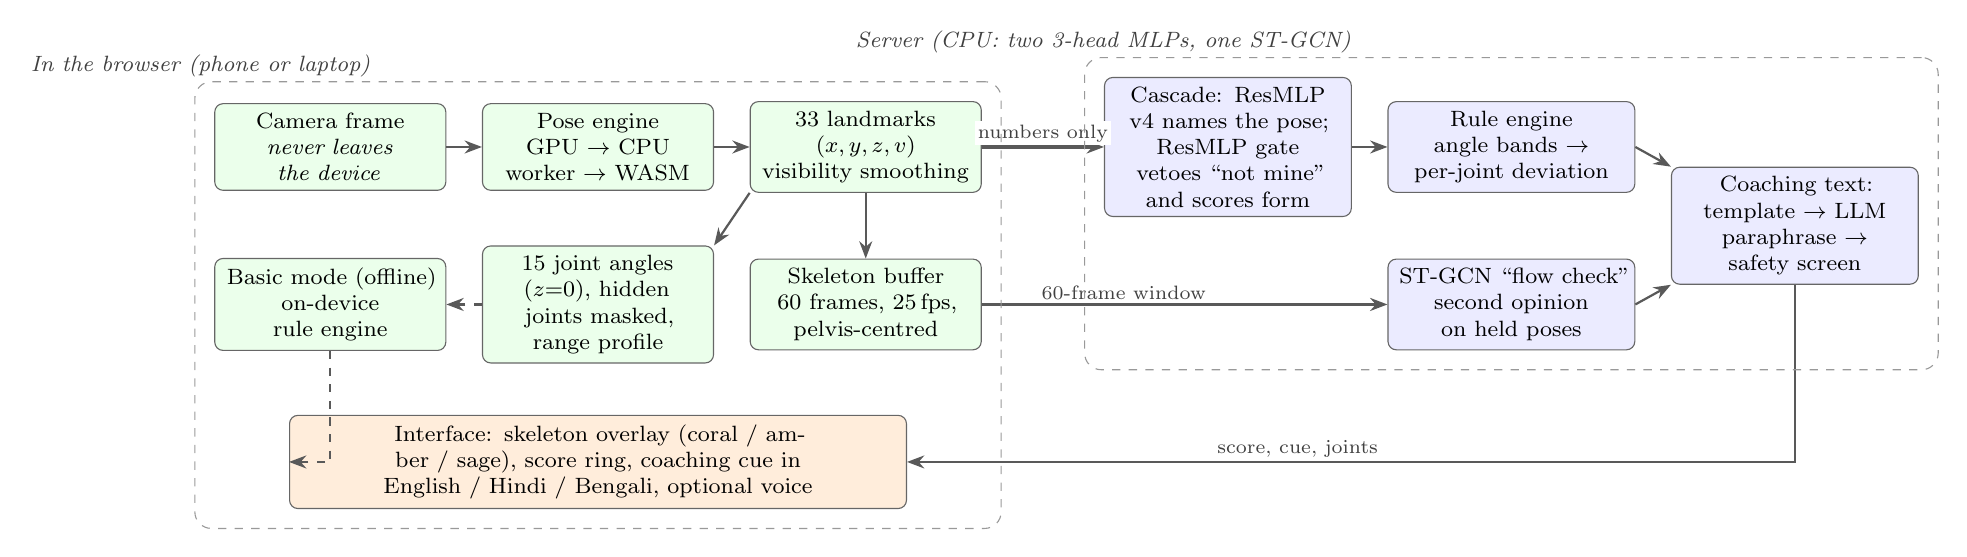
\begin{tikzpicture}[node distance=0pt, x=1cm, y=1cm]
\tikzset{
  dev/.style={rectangle,rounded corners=3pt,draw=black!60,fill=green!8,text width=2.7cm,align=center,minimum height=1.1cm,font=\footnotesize},
  srv/.style={rectangle,rounded corners=3pt,draw=black!60,fill=blue!8,text width=2.9cm,align=center,minimum height=1.1cm,font=\footnotesize},
  ui/.style={rectangle,rounded corners=3pt,draw=black!60,fill=orange!14,text width=7.6cm,align=center,minimum height=1.1cm,font=\footnotesize},
  ar/.style={-{Stealth[length=2.2mm]},thick,draw=black!65},
  lab/.style={font=\scriptsize,text=black!75,inner sep=1.2pt,fill=white},
  zone/.style={rectangle,rounded corners=6pt,draw=black!40,dashed,inner sep=7pt}
}
% ---- in the browser
\node[dev] (cam) at (0,0)    {Camera frame\\ \textit{never leaves the device}};
\node[dev] (eng) at (3.4,0)  {Pose engine\\ GPU $\rightarrow$ CPU worker $\rightarrow$ WASM};
\node[dev] (lm)  at (6.8,0)  {33 landmarks $(x,y,z,v)$\\ visibility smoothing};
\node[dev] (loc) at (0,-2.0) {Basic mode (offline)\\ on-device rule engine};
\node[dev] (ang) at (3.4,-2.0) {15 joint angles ($z{=}0$), hidden joints masked, range profile};
\node[dev] (buf) at (6.8,-2.0) {Skeleton buffer\\ 60 frames, 25\,fps, pelvis-centred};
\node[ui]  (uin) at (3.4,-4.0) {Interface: skeleton overlay (coral / amber / sage), score ring, coaching cue in English / Hindi / Bengali, optional voice};
% ---- on the server
\node[srv] (cas) at (11.4,0)    {Cascade: ResMLP \vfour{} names the pose; ResMLP gate vetoes ``not mine'' and scores form};
\node[srv] (rul) at (15.0,0)    {Rule engine\\ angle bands $\rightarrow$ per-joint deviation};
\node[srv] (stg) at (15.0,-2.0) {ST-GCN ``flow check''\\ second opinion on held poses};
\node[srv] (coa) at (18.6,-1.0) {Coaching text: template $\rightarrow$ LLM paraphrase $\rightarrow$ safety screen};
% ---- arrows
\draw[ar] (cam)--(eng); \draw[ar] (eng)--(lm);
\draw[ar] (lm.south west)--(ang.north east);
\draw[ar] (lm.south)--(buf.north);
\draw[ar,dashed] (ang.west)--(loc.east);
\draw[ar,line width=1.2pt] (lm.east)-- node[above,lab]{numbers only} (cas.west);
\draw[ar,line width=1.2pt] (buf.east)-- node[above,lab,pos=0.35]{60-frame window} (stg.west);
\draw[ar] (cas)--(rul);
\draw[ar] (rul.east)--(coa.north west);
\draw[ar] (stg.east)--(coa.south west);
\draw[ar] (coa.south) |- node[above,lab,pos=0.78]{score, cue, joints} (uin.east);
\draw[ar,dashed] (loc.south) |- (uin.west);
% ---- zones
\node[zone,fit=(cam)(eng)(lm)(loc)(ang)(buf)(uin),label={[lab,font=\footnotesize\itshape]above left:In the browser (phone or laptop)}] {};
\node[zone,fit=(cas)(rul)(stg)(coa),label={[lab,font=\footnotesize\itshape]above left:Server (CPU: two 3-head MLPs, one ST-GCN)}] {};
\end{tikzpicture}
}
\caption{AsanaAI architecture. Everything left of the network arrow runs in the browser: the camera frame is turned into 33 landmarks by a pose engine chosen automatically (Section~\ref{sec:deploy}), hidden joints are masked, and only landmark-derived numbers are sent. The server holds three small models and a rule engine; a rule-engine port in the browser keeps a basic mode working offline. Dashed arrows show the offline path.}
\label{fig:arch}
\end{figure}
AsanaAI is a web app (a progressive web app that also installs on a phone's home screen) with a public landing page and the practice screen. Fig.~\ref{fig:arch} shows the data flow.

\runin{On the device.} The browser opens the camera and a pose engine returns 33 landmarks $(x,y,z,v)$ per frame, where $v$ is the estimator's visibility. Visibility is smoothed with hysteresis so that a joint does not flicker between seen and hidden. From the landmarks the page computes 15 joint angles (Section~\ref{sec:features}) and, separately, a rolling 60-frame skeleton buffer resampled to 25\,fps. The camera frame itself is never uploaded; only numbers are sent: the 15-angle vector (with the user's calibration ranges, if any) and, for the sequence model, the buffered landmark coordinates, so the privacy promise on the landing page (``your video stays on your device'') is enforced by construction. A per-user calibration profile is kept in the browser's local storage (Section~\ref{sec:calib}).

\runin{On the server.} A CPU service (a Hugging Face Space) receives the angle vector at about one request every 1.5\,s. A cascade of two 3-head residual MLPs names the pose and decides whether it is ``not one of mine'' (Section~\ref{sec:cascade}); a rule engine compares the angles with each pose's reference bands and returns per-joint deviations; an ST-GCN scores 60-frame windows as a second opinion we call the \emph{flow check} (Section~\ref{sec:stgcn}). The coaching sentence is composed from reviewed templates and optionally paraphrased by a language model behind a safety screen (Section~\ref{sec:safety}). All three networks plus the rule engine fit in 324\,MB peak memory, and server compute is 7--9\,ms per request (median).

\runin{Two practice modes.} In \emph{free mode} nothing is selected and the server names whatever it recognises (the pose guide lists six reference poses); \emph{Guided mode} lets the user pick one of 8 target poses (Warrior II, Tree, Triangle, Chair, Downward Dog, Plank, Seated Easy, Corpse), shows the credited reference photo and measured joints, and replaces the score by a wrong-pose card if the camera sees another pose.

\runin{Languages and voice.} The interface, cues and optional speech are available in English, Hindi and Bengali.

\section{Data and Labels}\label{sec:data}
\subsection{Video corpus and cue-verified labels}
We collected 24 instructor-led yoga videos (12 original and 12 added later), 1{,}206{,}391 frames in total, and ran MediaPipe on every frame. Frame labels are \emph{cue-verified}: a frame is a positive example of a pose only if (i)~the instructor names that pose in the speech transcript (Whisper-large-v3 \cite{radford2023whisper}, English and Hindi), and (ii)~the app's own rule engine agrees with the name, and (iii)~the body is held steady. This yields about 80\,k positive frames; about 421\,k frames are labelled transition (the body is moving between poses) and about 705\,k are excluded as ambiguous. The point of the triple check is that no one of the three sources is trusted alone: an instructor may name a pose before or after the body reaches it, and labels from a rule engine alone would only teach a model to copy the rules.

\subsection{Features, and a train/serve mismatch}\label{sec:features}
The models see 15 joint angles computed from the 2-D landmarks (the $z$ coordinate is set to zero): left/right elbow, shoulder, hip, knee and ankle angles; left/right trunk angles; the neck angle; and left/right hip abduction. This is exactly what the browser can compute cheaply and what is sent. An audit showed that the original training table had been built with raw 3-D angles while the app serves zero-$z$ angles: the median per-feature gap was $14^\circ$, a pure train/serve skew \cite{sculley2015debt}. All training tables used here are rebuilt with the served recipe.

\subsection{Photo sets}
Photos supply the variety that 24 videos cannot. Commons-422 is a set of 422 freely licensed Wikimedia photos with a frozen test split of 103 (hash-split, fixed since 19 Sep 2026). Public photos are 6{,}616 photos from two public datasets: 2{,}634 labelled with our poses and 3{,}982 of poses outside our vocabulary, used as negatives; 4{,}931 are used for training and 1{,}685 are held out (1{,}037 of them are ``other poses''). Table~\ref{tab:data} summarises the data.
\begin{table}[t]
\centering\footnotesize
\caption{Data used in this paper.}\label{tab:data}
\begin{tabularx}{\columnwidth}{@{}lX@{}}
\toprule
Item & Size / detail \\ \midrule
Training videos & 24, 1{,}206{,}391 frames; $\sim$80\,k positive / $\sim$421\,k transition / $\sim$705\,k excluded \\
Features & 15 zero-$z$ joint angles per frame (MLP); 60$\times$33$\times$3 landmark windows (ST-GCN) \\
Commons-422 & 422 photos; frozen test split 103 \\
Public photos & 6{,}616 (4{,}931 train / 1{,}685 held out, of which 1{,}037 are ``other poses'') \\
ST-GCN windows & 24 videos, 8{,}002 windows (60 frames, stride 12), 3 folds by video \\ \bottomrule
\end{tabularx}
\end{table}

\subsection{Evaluation protocol}
A number counts only if it was measured on data the model never trained on. A pose \emph{passes} if recall $\ge0.70$ and precision $\ge0.70$ with at least 10 held-out photos (5 on the tiny frozen set; 20 windows for the ST-GCN). A \emph{false alarm} is a photo of a pose that is not one of the app's poses that the system names as one of them (lower is better). Sequence models are scored on three folds split by video, so the model never sees the person or room it is tested on. The trainers' own validation accuracy (90--98\%) comes from a random split and is never quoted as a result.

\section{Models}\label{sec:models}
\begin{figure}[t]
\centering
\begin{minipage}[b]{0.50\textwidth}\centering
\resizebox{\linewidth}{!}{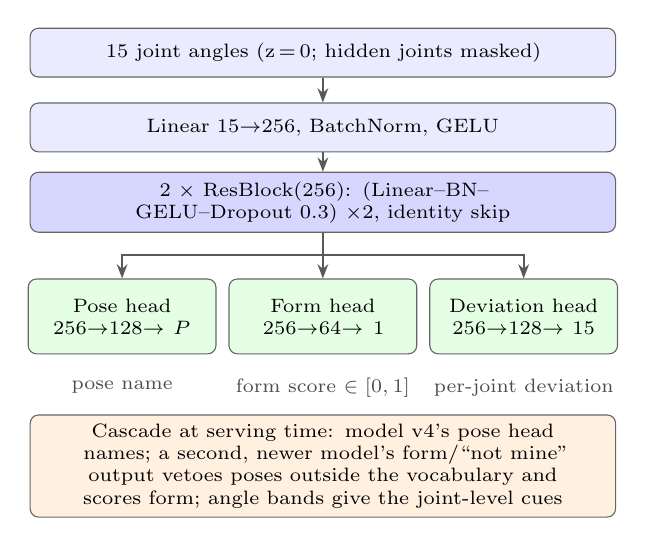
\begin{tikzpicture}[x=1cm,y=1cm]
\tikzset{
  nb/.style={rectangle,rounded corners=3pt,draw=black!60,fill=blue!8,text width=7.2cm,align=center,minimum height=0.62cm,font=\scriptsize},
  hd/.style={rectangle,rounded corners=3pt,draw=black!60,fill=green!10,text width=2.15cm,align=center,minimum height=0.95cm,font=\scriptsize},
  ar/.style={-{Stealth[length=1.8mm]},thick,draw=black!65}
}
\node[nb] (in) at (0,0) {15 joint angles (z\,=\,0; hidden joints masked)};
\node[nb] (l1) at (0,-0.95) {Linear 15$\rightarrow$256, BatchNorm, GELU};
\node[nb,fill=blue!16] (rb) at (0,-1.9) {2 $\times$ ResBlock(256): (Linear--BN--GELU--Dropout 0.3) $\times 2$, identity skip};
\node[hd] (h1) at (-2.55,-3.35) {Pose head\\ 256$\rightarrow$128$\rightarrow P$};
\node[hd] (h2) at (0,-3.35) {Form head\\ 256$\rightarrow$64$\rightarrow 1$};
\node[hd] (h3) at (2.55,-3.35) {Deviation head\\ 256$\rightarrow$128$\rightarrow 15$};
\draw[ar] (in)--(l1); \draw[ar] (l1)--(rb);
\draw[ar] (rb.south) -- ++(0,-0.28) -| (h1.north);
\draw[ar] (rb.south) -- (h2.north |- rb.south) -- (h2.north);
\draw[ar] (rb.south) -- ++(0,-0.28) -| (h3.north);
\node[font=\scriptsize,text=black!70] at (-2.55,-4.25) {pose name};
\node[font=\scriptsize,text=black!70] at (0,-4.25) {form score $\in[0,1]$};
\node[font=\scriptsize,text=black!70] at (2.55,-4.25) {per-joint deviation};
% cascade
\node[nb,fill=orange!12,text width=7.2cm] (cas) at (0,-5.25) {Cascade at serving time: model \vfour{}'s pose head names; a second, newer model's form/``not mine'' output vetoes poses outside the vocabulary and scores form; angle bands give the joint-level cues};
\end{tikzpicture}
}\\[2pt]
{\footnotesize (a) The 3-head residual MLP and the cascade.}
\end{minipage}\hfill
\begin{minipage}[b]{0.47\textwidth}\centering
\resizebox{\linewidth}{!}{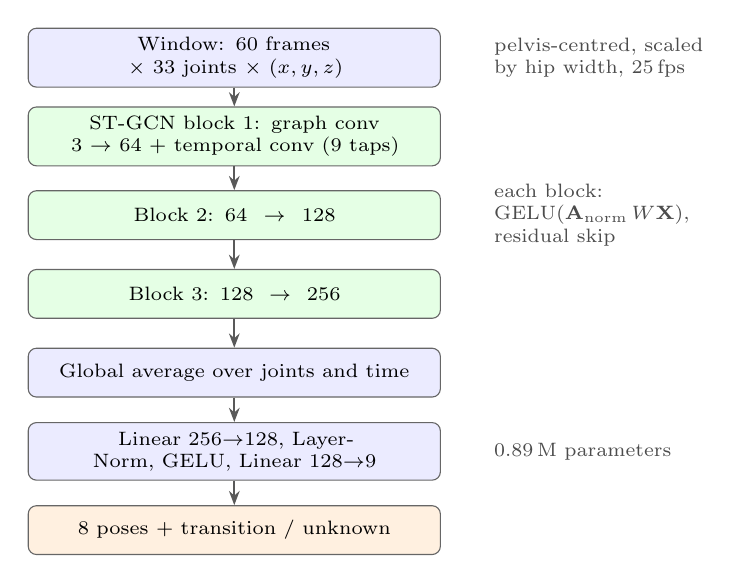
\begin{tikzpicture}[x=1cm,y=1cm]
\tikzset{
  nb/.style={rectangle,rounded corners=3pt,draw=black!60,fill=blue!8,text width=5.0cm,align=center,minimum height=0.62cm,font=\scriptsize},
  ar/.style={-{Stealth[length=1.8mm]},thick,draw=black!65},
  an/.style={font=\scriptsize,text=black!70,text width=2.7cm,align=left}
}
\node[nb] (in) at (0,0) {Window: 60 frames $\times$ 33 joints $\times$ $(x,y,z)$};
\node[nb,fill=green!10] (b1) at (0,-1.0) {ST-GCN block 1: graph conv $3\!\rightarrow\!64$ + temporal conv (9 taps)};
\node[nb,fill=green!10] (b2) at (0,-2.0) {Block 2: $64\!\rightarrow\!128$};
\node[nb,fill=green!10] (b3) at (0,-3.0) {Block 3: $128\!\rightarrow\!256$};
\node[nb] (gp) at (0,-4.0) {Global average over joints and time};
\node[nb] (fc) at (0,-5.0) {Linear 256$\rightarrow$128, LayerNorm, GELU, Linear 128$\rightarrow$9};
\node[nb,fill=orange!12] (out) at (0,-6.0) {8 poses + transition / unknown};
\foreach \a/\b in {in/b1,b1/b2,b2/b3,b3/gp,gp/fc,fc/out}{\draw[ar] (\a)--(\b);}
\node[an] at (4.65,-0.0) {pelvis-centred, scaled by hip width, 25\,fps};
\node[an] at (4.65,-2.0) {each block: $\mathrm{GELU}(\mathbf{A}_{\mathrm{norm}}\,W\mathbf{X})$, residual skip};
\node[an] at (4.65,-5.0) {0.89\,M parameters};
\end{tikzpicture}
}\\[2pt]
{\footnotesize (b) The ST-GCN sequence model (``flow check'').}
\end{minipage}
\caption{The two learned models. $P$ is the number of pose classes. For $P\approx22$ the MLP has about 0.36\,M parameters; the nine-class ST-GCN has about 0.89\,M (both counted from the model definitions).}
\label{fig:models}
\end{figure}

\subsection{3-head residual MLP}
The pose model takes the 15-angle vector (Section~\ref{sec:features}) and passes it through a 256-unit input layer (Linear, batch normalisation \cite{ioffe2015bn}, GELU \cite{hendrycks2016gelu}) and two residual blocks \cite{he2016resnet} of width 256 (two Linear--BN--GELU--Dropout stages with an identity skip). Three heads share this trunk (Fig.~\ref{fig:models}a): a \emph{pose head} (256$\to$128$\to P$ logits), a \emph{form head} (256$\to$64$\to1$, a correctness probability), and a \emph{deviation head} (256$\to$128$\to$15 per-joint deviations). Sharing the trunk makes one forward pass of about 0.36\,M parameters answer ``which pose, how well, which joints'' in a few milliseconds on a CPU.

\subsection{The cascade: one model names, another vetoes}\label{sec:cascade}
Through the original decision path, a rule engine overrode the MLP on every disagreement, so replacing the MLP with a better one changed nothing (identical to rules-only, Table~\ref{tab:policy}). We therefore split the roles. The \emph{namer} is the earlier photo-trained 3-head MLP (\vfour{}), whose top pose is the answer. The \emph{gate} is a newer 3-head MLP of the same architecture trained on the cue-verified video table plus training photos and photos of other poses (labelled transition/unknown); it answers ``is this one of my poses at all?'' and supplies the form score. The rule is fixed in advance: the answer is \vfour{}'s top pose unless the gate's top class is transition/unknown, in which case the system says it does not recognise a pose. This is a reject option in the sense of selective classification \cite{geifman2017selective}, applied at the system level. The policy was chosen on a validation half of the held-out photos and confirmed on the untouched half (Section~\ref{sec:results}).

\subsection{Rule engine and per-joint cues}
Each pose has a table of angle bands (e.g.\ for Downward Dog: knee $\in[110^\circ,180^\circ]$, shoulder $\in[95^\circ,180^\circ]$, hip $\in[20^\circ,140^\circ]$). The deviation of a joint is the distance in degrees outside its band (0 if inside), and the rule score is $1-\overline{d}/45^\circ$ clipped to $[0,1]$. Because the learned deviation head turned out to be weak (Section~\ref{sec:results}), the per-joint cue and the colour of each limb in the skeleton overlay come from these bands wherever a pose has them (17 of the 19 poses): coral if a joint is more than $15^\circ$ outside, amber above $7^\circ$, sage otherwise (Fig.~\ref{fig:occ}a). Two poses, Tree and Lunge, have no bands. Until 2026-10-07 the cascade fell back to the learned head for them, so a correct Tree could show a coral leg (Fig.~\ref{fig:occ}d); we found this while verifying the calibration feature, and the deployed system now reports no per-joint deviations for these two poses and draws neutral limbs (Section~\ref{sec:limits}).

\subsection{ST-GCN ``flow check''}\label{sec:stgcn}
The sequence model treats a 60-frame window as a graph signal on the 33-joint MediaPipe skeleton. Coordinates are centred on the pelvis and divided by the hip width. Each of three ST-GCN blocks \cite{yan2018stgcn} applies a graph convolution with the symmetric-normalised skeleton adjacency $\mathbf{A}_{\mathrm{norm}}=\mathbf{D}^{-1/2}(\mathbf{A}+\mathbf{I})\mathbf{D}^{-1/2}$ (a $1{\times}1$ projection followed by aggregation over neighbours) and a 9-tap temporal convolution, with GELU and a residual connection; channels grow $3\to64\to128\to256$, features are averaged over joints and time, and a two-layer head outputs eight target poses plus transition/unknown (Fig.~\ref{fig:models}b). The app shows a flow-check answer only if its confidence reaches 0.70 (0.55 for child's pose); otherwise the UI shows ``static check'', and the per-frame cascade alone names the pose and scores form.

\runin{The input-rate contract.} The model is trained on 60 consecutive native-rate frames ($\approx$2.4\,s at 25\,fps). An early version of the web app fed its buffer one frame per finished server round trip (at most 2\,fps), so its ``60 frames'' spanned 30--120\,s and the model looked broken. The app now fills a time-based buffer from every camera frame and resamples it to 25\,fps; Section~\ref{sec:results} quantifies why this matters.

\section{Occlusion, Personalisation and Safe Coaching}\label{sec:occ}
\begin{figure}[t]
\centering
\begin{subfigure}[t]{0.175\textwidth}\centering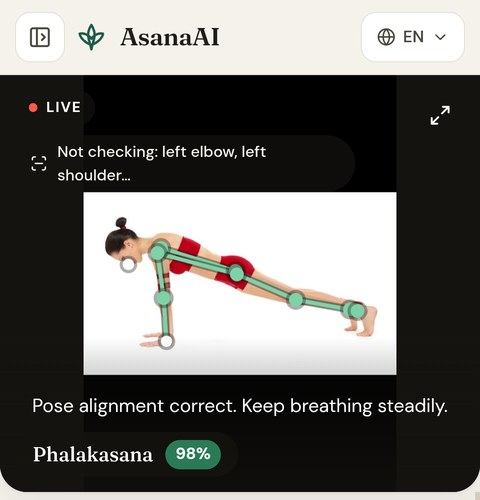
\includegraphics[width=\linewidth]{figures/oc_plank_hidden.jpg}\caption{Hidden joints are not judged}\end{subfigure}\hfill
\begin{subfigure}[t]{0.175\textwidth}\centering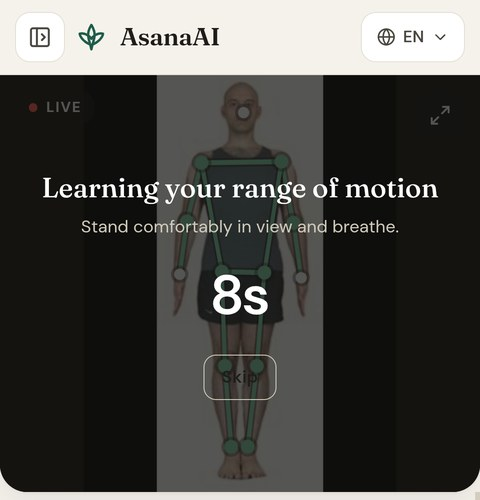
\includegraphics[width=\linewidth]{figures/cal_countdown.jpg}\caption{Calibration: 15\,s countdown}\end{subfigure}\hfill
\begin{subfigure}[t]{0.175\textwidth}\centering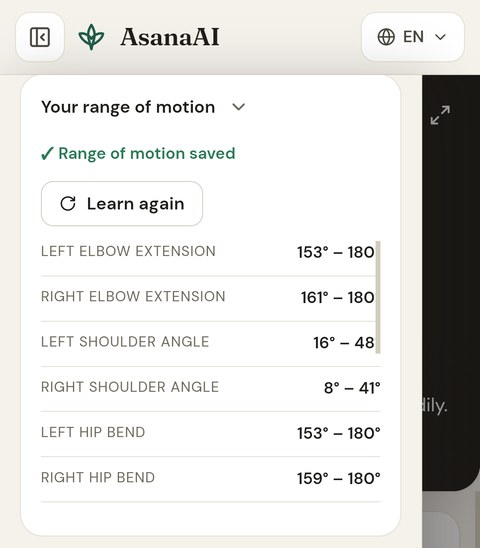
\includegraphics[width=\linewidth]{figures/cal_range.jpg}\caption{Saved range of motion}\end{subfigure}\hfill
\begin{subfigure}[t]{0.175\textwidth}\centering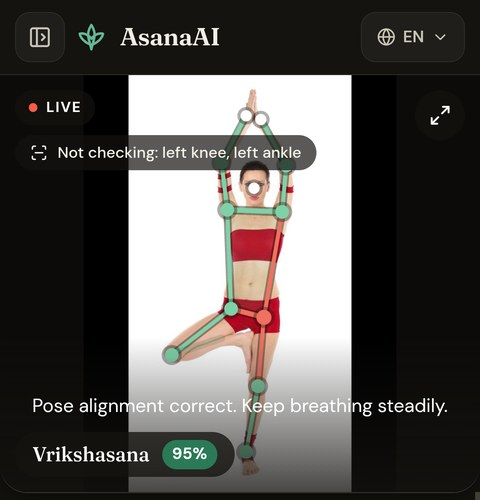
\includegraphics[width=\linewidth]{figures/oc_tree_hidden.jpg}\caption{Failure: false coral leg}\end{subfigure}\hfill
\begin{subfigure}[t]{0.175\textwidth}\centering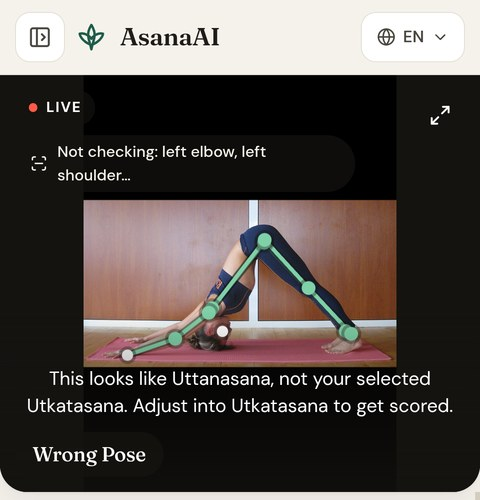
\includegraphics[width=\linewidth]{figures/fail_dog.jpg}\caption{Failure: wrong name}\end{subfigure}
\caption{Live screenshots of the deployed app on a POCO M7 Pro over USB, with a credited Wikimedia photo standing in for the camera (no live person). (a)~Plank, guided mode: visible limbs are sage (inside their angle bands) and the chip ``Not checking: left elbow, left shoulder'' names joints the camera cannot see, which are drawn faint and neither scored nor coached. (b)~Calibration asks the user to stand comfortably for 15\,s. (c)~The learned per-joint ranges are saved on the device (the still photo yields narrow ranges). Two failures shown on purpose: (d)~a correct Tree (guided, dark theme) with a coral standing leg, captured before the fix: Tree has no angle bands, so its joint colours then came from the learned deviation head, which is unreliable; the deployed app now draws neutral limbs for Tree and Lunge (Section~\ref{sec:models}); (e)~a Downward Dog photo named Uttanasana (a forward fold), after which guided mode answers ``Wrong Pose''. Photos: Kennguru (a, d), Witold Fitz-Simon (b, c; CC BY-SA 2.5), Iveto (e); CC BY 3.0 unless noted, via Wikimedia Commons.}
\label{fig:occ}
\end{figure}

\subsection{Visibility-aware scoring}
An audit of the first version showed that the server's mesh-recovery branch was never wired (nothing sent it data and no such model was deployed), and what actually ran for hidden joints was a left--right mirror: exact for symmetric stances, wrong for asymmetric ones. In Tree pose the raised foot was placed on the floor, off by 0.23 of the frame height, and still reported as ``recovered''. Meanwhile the joint angles were always computed from the raw landmarks, so a hidden joint could still produce a confident wrong score and cue.

We replaced guessing with abstaining. Joints whose landmark visibility is low (smoothed with hysteresis in the browser) are neither scored nor coached; the interface lists what it is not checking (Fig.~\ref{fig:occ}a) and draws hidden limbs at 25\% opacity. The map from hidden joint to affected angle features was checked against the Python angle code by perturbation (0 visibility errors). A known limit remains: the pose name can still be influenced by a hallucinated hidden joint; only scoring and coaching are masked.

\subsection{Would mesh recovery do better? CLIFF versus the mirror}
Mirroring is crude, so we asked whether CLIFF \cite{li2022cliff} (a ResNet-50 model that predicts an SMPL body \cite{loper2015smpl} from the full frame) recovers hidden joints better. On 70 real yoga frames in four poses, with MediaPipe on the clean frame as the reference, a grey box hid one limb (left leg, right arm or both feet; 141 cases) and the hidden joints were recovered four ways. Table~\ref{tab:cliff} gives the errors.
\begin{table}[t]
\centering\footnotesize\setlength{\tabcolsep}{3pt}
\caption{Recovering hidden joints (141 cases; lower is better). Errors are relative to MediaPipe on the clean frame; NME is 2-D distance over torso length. Bold: better of the compared methods within each subset.}\label{tab:cliff}
\begin{tabular}{@{}llrrr@{}}
\toprule
Subset ($n$) & Method & Med.\ angle & Mean angle & Med.\ NME \\ \midrule
All (141) & raw & $17.9^\circ$ & $38.9^\circ$ & 0.291 \\
 & mirror & $8.6^\circ$ & $20.2^\circ$ & \textbf{0.152} \\
 & CLIFF & $\mathbf{5.8^\circ}$ & $\mathbf{16.8^\circ}$ & 0.185 \\
 & CLIFF aligned & $7.0^\circ$ & $22.0^\circ$ & 0.179 \\ \midrule
Symmetric (117) & mirror & $\mathbf{5.2^\circ}$ & $13.8^\circ$ & \textbf{0.131} \\
 & CLIFF & $6.1^\circ$ & $\mathbf{11.0^\circ}$ & 0.173 \\
Tree, asym.\ (24) & mirror & $20.1^\circ$ & $51.2^\circ$ & 0.470 \\
 & CLIFF & $\mathbf{4.8^\circ}$ & $\mathbf{44.8^\circ}$ & \textbf{0.357} \\
Left leg (47) & mirror & $16.2^\circ$ & $33.5^\circ$ & \textbf{0.214} \\
 & CLIFF & $\mathbf{6.2^\circ}$ & $\mathbf{12.7^\circ}$ & 0.270 \\
Right arm (47) & mirror & $\mathbf{4.9^\circ}$ & $\mathbf{11.9^\circ}$ & \textbf{0.092} \\
 & CLIFF & $15.1^\circ$ & $30.7^\circ$ & 0.210 \\
Both feet (47) & mirror ($=$raw) & $6.1^\circ$ & $15.1^\circ$ & 0.199 \\
 & CLIFF & $\mathbf{4.7^\circ}$ & $\mathbf{6.9^\circ}$ & \textbf{0.143} \\ \bottomrule
\end{tabular}
\end{table}
Neither method dominates. The mirror is better where the body really is symmetric (arms, mountain, seated) and has the lowest median landmark error overall; CLIFF is better for legs, for both feet hidden and for the asymmetric Tree pose, and its median joint-angle error is $5.8^\circ$ versus $8.6^\circ$. But CLIFF costs 164\,ms per image on two CPU threads (18.7\,ms on a T4 GPU) and, decisively, needs the image, which the app never sends. We therefore do not ship it and keep the abstain policy. Caveats: 141 cases from 70 frames, one asymmetric pose, a synthetic occluder, a MediaPipe reference rather than motion capture, and a neutral body-model stand-in for an unavailable initialisation file.

\subsection{Personal range-of-motion calibration}\label{sec:calib}
Bodies differ: a joint inside its owner's comfortable range is ``different'', not ``wrong''. At camera start the app offers a 15-second calibration (Fig.~\ref{fig:occ}b): the user stands comfortably in view while the 15 joint angles are recorded. For each joint the profile stores the observed minimum and maximum widened by $15^\circ$ (clamped to $[0^\circ,180^\circ]$) and the mean as the resting angle; if fewer than 20 frames were captured it is discarded rather than ``pretend we calibrated''. The profile lives only in the browser's local storage (Fig.~\ref{fig:occ}c); each request carries the numbers. On the server, a joint whose angle lies inside its personal range has its deviation set to zero, and a personal form score is computed that closes the fraction of the gap to a perfect score that the forgiven deviation represents; it is therefore never lower than the universal score, and equal when nothing is forgiven. The UI shows it as ``For your body'' beside the universal score. We verified the mechanism against the deployed server with a hand-built skeleton (angles from the app's own function; both hip deviations $56^\circ$ from their bands, universal score 0.924). Without a profile the response carries no personal score; a profile not containing the current angles leaves it at 0.924; one containing the left hip's angle zeroes that deviation (0.962); both hips give 1.000; the universal score never changed. A profile spanning $0^\circ$--$180^\circ$ for every joint also gives 1.000, which shows how much a poor profile can forgive. The feature has not been validated with users or clinicians (Section~\ref{sec:limits}).

\subsection{Safe, multilingual coaching}\label{sec:safety}
The cue sentence goes through three stages. (1)~A symbolic stage picks the joint furthest outside its band and a reviewed template for it in English, Hindi or Bengali. (2)~Optionally, a hosted language model (a 27-billion-parameter Qwen model, temperature 0.2) paraphrases the template and may only rewrite it. (3)~A post-generation screen discards the paraphrase and keeps the template if it contains any of ``push'', ``force'', ``hurt'', ``pain'', ``stretch more'' or ``further''. A cue that is delivered and produces no measured improvement escalates: the second time it adds how many degrees off the user is, and from the third time it backs off (``ease out of the shape and reset; come back only as far as feels comfortable today''), because a cue that failed twice usually means the range is not available today. A lesson from operating this stage: when the provider retired the model name we had configured, every request silently fell back to the template and the failure looked identical to success until the response was found to be byte-identical to the template. The fallback is safe, which is exactly why a silent one is dangerous; the code now logs every non-200 answer.

\section{Deployment on Real Phones}\label{sec:deploy}
\begin{figure}[t]
\centering
\resizebox{0.48\textwidth}{!}{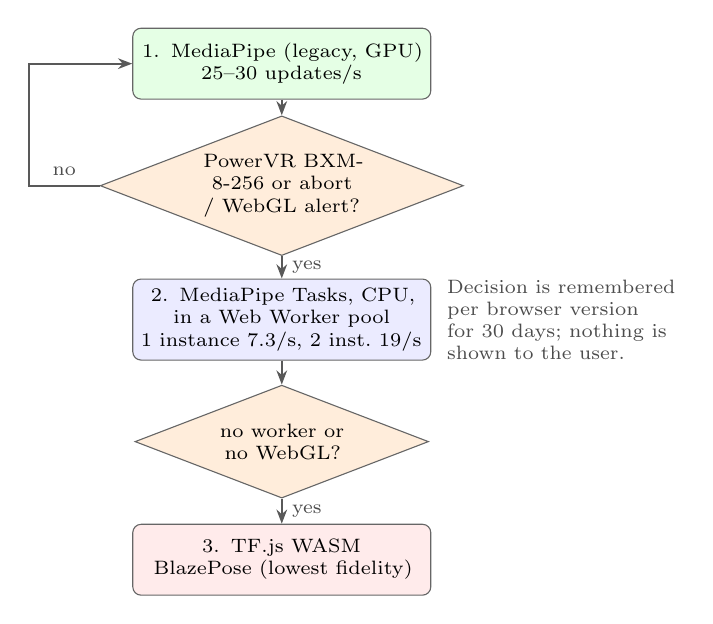
\begin{tikzpicture}[x=1cm,y=1cm]
\tikzset{
  nb/.style={rectangle,rounded corners=3pt,draw=black!60,fill=blue!8,text width=3.55cm,align=center,minimum height=0.9cm,font=\scriptsize},
  nd/.style={diamond,aspect=2.6,draw=black!60,fill=orange!14,text width=2.3cm,align=center,inner sep=1pt,font=\scriptsize},
  ar/.style={-{Stealth[length=1.8mm]},thick,draw=black!65},
  lb/.style={font=\scriptsize,text=black!70}
}
\node[nb,fill=green!10] (e1) at (0,0) {1. MediaPipe (legacy, GPU)\\ 25--30 updates/s};
\node[nd] (d1) at (0,-1.55) {PowerVR BXM-8-256 or abort / WebGL alert?};
\node[nb] (e2) at (0,-3.25) {2. MediaPipe Tasks, CPU, in a Web Worker pool\\ 1 instance 7.3/s, 2 inst.\ 19/s};
\node[nd] (d2) at (0,-4.8) {no worker or no WebGL?};
\node[nb,fill=red!8] (e3) at (0,-6.3) {3. TF.js WASM BlazePose (lowest fidelity)};
\draw[ar] (e1)--(d1); \draw[ar] (d1)--node[right,lb]{yes}(e2); \draw[ar] (e2)--(d2); \draw[ar] (d2)--node[right,lb]{yes}(e3);
\draw[ar] (d1.west) -- node[above,lb]{no} ++(-0.9,0) |- ($(e1.west)+(0,-0.0)$) ;
\node[lb,text width=2.9cm,align=left] at (3.55,-3.25) {Decision is remembered per browser version for 30 days; nothing is shown to the user.};
\end{tikzpicture}
}
\caption{The pose-engine fallback ladder. The choice is automatic, remembered per browser version for up to 30 days, and invisible to the user.}
\label{fig:ladder}
\end{figure}
\runin{The failure.} On a POCO M7 Pro (MediaTek Dimensity 7025, PowerVR BXM-8-256 GPU, Android 16, Chrome 154) the web app showed a raw ``Failed to create WebGL canvas context'' alert. This is not ``no WebGL'': Chrome creates WebGL2, WebGL1 and OffscreenCanvas contexts fine. The legacy MediaPipe pose engine then aborts inside the GPU driver (a shader-uniform assertion in its image scaler) and every later frame throws; MediaPipe Tasks with the GPU delegate runs in 16\,ms per frame but returns no poses. Driver problems of this GPU family are discussed on the vendor's developer forum,\footnote{\url{https://forums.imgtec.com/t/bxm-8-256-long-list-of-driver-issues/3891}} and the alert itself is a alert box inside MediaPipe's script.\footnote{\url{https://github.com/google/mediapipe/issues/2381}} Because fixes must be automatic, we measured candidate engines over USB with the Chrome DevTools Protocol, touching only a tab we create.

\runin{The ladder.} The app tries MediaPipe on the GPU; if the renderer is the known-bad chip (recognised at page load) or the engine aborts or raises the alert, it switches to MediaPipe Tasks on the CPU inside a Web Worker (a second MediaPipe module cannot share the page with the legacy one because of a global-namespace collision, hence the worker); if no worker or WebGL is available it falls back to TensorFlow.js \cite{smilkov2019tfjs} with a WebAssembly BlazePose (Fig.~\ref{fig:ladder}). Table~\ref{tab:engines} gives what we measured.
\begin{table}[t]
\centering\footnotesize
\caption{Pose engines measured on the POCO M7 Pro (lite models unless stated).}\label{tab:engines}
\begin{tabularx}{\columnwidth}{@{}Xr@{}}
\toprule
Engine / configuration & Measured \\ \midrule
Legacy MediaPipe, GPU (PowerVR BXM-8-256) & aborts in driver \\
MediaPipe Tasks, GPU delegate & 16\,ms, no poses \\
Tasks, CPU, image mode & $\sim$176\,ms/frame \\
Tasks, CPU, video mode (lite / full) & $\sim$80 / $\sim$117\,ms \\
$\ldots$ in a Web Worker, round trip & 85--95\,ms \\
Worker pool, 1 / 2 / 3 instances & 7.3 / 19 / 24 results/s \\
TF.js WASM BlazePose (last resort) & $\sim$95\,ms; $4.2$--$6.7^\circ$ mean angle gap \\ \bottomrule
\end{tabularx}
\end{table}
A single worker gave 7.3 results/s; phones with at least six cores now run two instances and alternate frames (late answers for older frames are dropped), which raised the skeleton from about 8--10 to about 22 updates/s in the running app. The last-resort engine is lower in fidelity: against the CPU engine its mean joint-angle difference was $4.2$--$6.7^\circ$ (worst $27^\circ$) and it missed a plank. On a desktop, the GPU and CPU engines differed by $2.4^\circ$ (Tree), $2.5^\circ$ (Cobra) and $4.8^\circ$ (Warrior~II) on the same photos. The same fallback also worked in a second browser (Brave) that masks the GPU name, where recognition up front is impossible and the reactive path took over after the driver abort, then drew the skeleton and recognised Warrior~II at 98\% (one photo).

\runin{Offline and degraded operation.} When the server is unreachable, the browser falls back to \emph{basic mode}: a TypeScript port of the rule engine and coaching templates. We proved the port against the Python original with generated cases: 10{,}000 frame cases and 2{,}500 coaching-text cases over 21 poses, 0 mismatches. Basic mode is rules only---no MLP, no gate, no ST-GCN, no language model---so its pose naming equals the ``rules only'' row of Table~\ref{tab:policy}, not the cascade; the interface says so and says why (offline, server waking, reconnecting). The first answer of a session is local so the user never waits for a sleeping server, API calls time out after 9\,s, and pose and score refresh about every 1.5\,s (every 10\,s in the first version).

\section{Results}\label{sec:results}
All numbers below were measured on data the models never trained on (Section~\ref{sec:data}); where a caveat applies it is stated next to the number.

\subsection{Naming the pose from one frame}
\runin{Progress over model generations.} Table~\ref{tab:posehead} follows the pose model from the first (about two-month-old) model to the current one. On the held-out public photos the earliest models passed no pose; the current gate model passes three with 22.6\% false alarms. The 86--90\% that two September models score on all 422 Commons photos is deliberately omitted because they were trained on most of those photos.
\begin{table}[t]
\centering\footnotesize
\caption{Pose-head generations on clean tests (bold: best in column). Frozen Commons-103: none of these models trained on those photos (the new model is scored out-of-fold). Held-out public photos: 1{,}685 (1{,}037 other poses); \vfour{} may have seen similar public images, which can only flatter it.}\label{tab:posehead}
\begin{tabular}{@{}lrrrr@{}}
\toprule
 & \multicolumn{2}{c}{Frozen Commons-103} & \multicolumn{2}{c}{Held-out public} \\
Model & Overall & Macro rec. & Poses pass & False alarm \\ \midrule
19 Jul original & 23.3\% & 17.5\% & 0 & 75.0\% \\
3 Sep retrain & 13.6\% & 11.1\% & 0 & 64.5\% \\
21 Sep \vfour{} (was live) & \textbf{60.2\%} & \textbf{64.8\%} & 1 & 81.5\% \\
New (gate model) & 49.5\% & 58.0\% & \textbf{3} & \textbf{22.6\%} \\ \bottomrule
\end{tabular}
\end{table}

\runin{The decision path matters more than the model.} Table~\ref{tab:policy} and Fig.~\ref{fig:charts}a compare decision policies on the 1{,}685 held-out public photos using the real production functions. Through the original path (rule engine wins every disagreement) a new MLP changed nothing: identical to rules-only (36.9\%, 78.3\% false alarms, no pose passing). The cascade reaches 78.9\% with 20.8\% false alarms and seven poses at recall and precision $\ge0.70$ (chair, corpse, downward dog, tree, triangle, upward dog, Warrior~II). The policy was chosen on a validation half only (79.3\%, 20.1\%, 3 poses) and confirmed on the untouched half (78.6\%, 21.6\%, 4 poses: corpse, downward dog, tree, Warrior~II). On the wild frozen-103 set the cascade scores 55.3\% against 37.9--40.8\% before; \vfour{} alone is better at pure naming there (60.2\%), so the cascade gives up about five photos of naming accuracy for about 60 points fewer false alarms elsewhere. Through the real frame-analysis endpoint with the real models, switching the cascade off reproduced production exactly and switching it on reproduced 78.9\%/20.8\%/7, agreeing with the offline policy on 100\% of requests; a replay against the live Space gave 78.1\%/21.8\%/7 (16 of 1{,}685 requests were rejected by the host's rate limiter under an 8-thread stress test).
\begin{table}[t]
\centering\footnotesize\setlength{\tabcolsep}{4pt}
\caption{Decision policies on the 1{,}685 held-out public photos (bold: best in column). False alarm: a photo of another pose named as one of ours (lower is better).}\label{tab:policy}
\begin{tabular}{@{}lrrr@{}}
\toprule
Policy & Overall & False alarm & Poses pass \\ \midrule
Production before (\vfour{} + rules) & 36.9\% & 78.3\% & 0 \\
New model + rules & 36.9\% & 78.3\% & 0 \\
Rules only & 36.9\% & 78.3\% & 0 \\
\vfour{} alone & 42.9\% & 81.5\% & 1 \\
Average of both MLPs & 65.2\% & 47.7\% & 5 \\
Veto lifted when rules agree & 65.9\% & 42.3\% & 5 \\
Cascade (\vfour{} names, new model vetoes) & \textbf{78.9\%} & \textbf{20.8\%} & \textbf{7} \\ \bottomrule
\end{tabular}
\end{table}

\begin{figure}[t]
\centering
\begin{subfigure}[t]{0.32\textwidth}\centering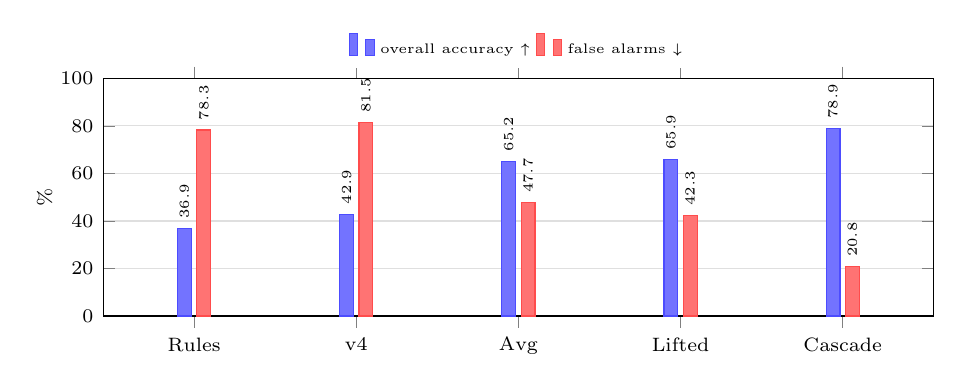
\begin{tikzpicture}
\begin{axis}[ybar,bar width=5pt,width=\linewidth,height=4.6cm,ymin=0,ymax=100,ylabel={\%},ylabel style={font=\scriptsize,yshift=-4pt},
  symbolic x coords={Rules,v4,Avg,Lifted,Cascade},xtick=data,x tick label style={font=\scriptsize},y tick label style={font=\scriptsize},
  legend style={font=\tiny,at={(0.5,1.04)},anchor=south,legend columns=2,draw=none},enlarge x limits=0.14,ymajorgrids,grid style={gray!25},
  nodes near coords,nodes near coords style={font=\tiny,/pgf/number format/fixed,/pgf/number format/precision=1},every node near coord/.append style={rotate=90,anchor=west}]
\addplot[fill=blue!55,draw=blue!70] coordinates {(Rules,36.9)(v4,42.9)(Avg,65.2)(Lifted,65.9)(Cascade,78.9)};
\addplot[fill=red!55,draw=red!70] coordinates {(Rules,78.3)(v4,81.5)(Avg,47.7)(Lifted,42.3)(Cascade,20.8)};
\legend{overall accuracy $\uparrow$,false alarms $\downarrow$}
\end{axis}
\end{tikzpicture}
\caption{Decision policies (held-out public photos)}\end{subfigure}\hfill
\begin{subfigure}[t]{0.32\textwidth}\centering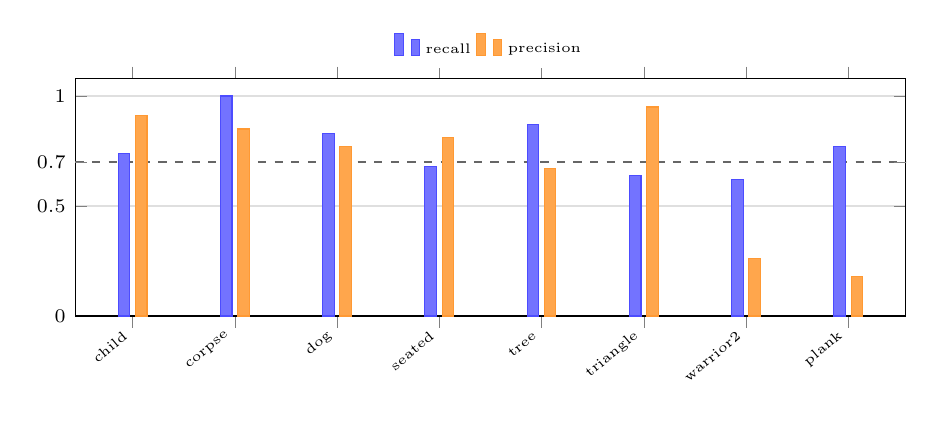
\begin{tikzpicture}
\begin{axis}[ybar,bar width=4.2pt,width=\linewidth,height=4.6cm,ymin=0,ymax=1.08,
  symbolic x coords={child,corpse,dog,seated,tree,triangle,warrior2,plank},xtick=data,x tick label style={font=\tiny,rotate=40,anchor=east},y tick label style={font=\scriptsize},
  legend style={font=\tiny,at={(0.5,1.04)},anchor=south,legend columns=2,draw=none},enlarge x limits=0.08,ymajorgrids,grid style={gray!25},
  extra y ticks={0.7},extra y tick style={grid=major,grid style={dashed,black!60},tick label style={font=\tiny}}]
\addplot[fill=blue!55,draw=blue!70] coordinates {(child,0.74)(corpse,1.00)(dog,0.83)(seated,0.68)(tree,0.87)(triangle,0.64)(warrior2,0.62)(plank,0.77)};
\addplot[fill=orange!70,draw=orange!80] coordinates {(child,0.91)(corpse,0.85)(dog,0.77)(seated,0.81)(tree,0.67)(triangle,0.95)(warrior2,0.26)(plank,0.18)};
\legend{recall,precision}
\end{axis}
\end{tikzpicture}
\caption{ST-GCN, held-out videos, per pose}\end{subfigure}\hfill
\begin{subfigure}[t]{0.32\textwidth}\centering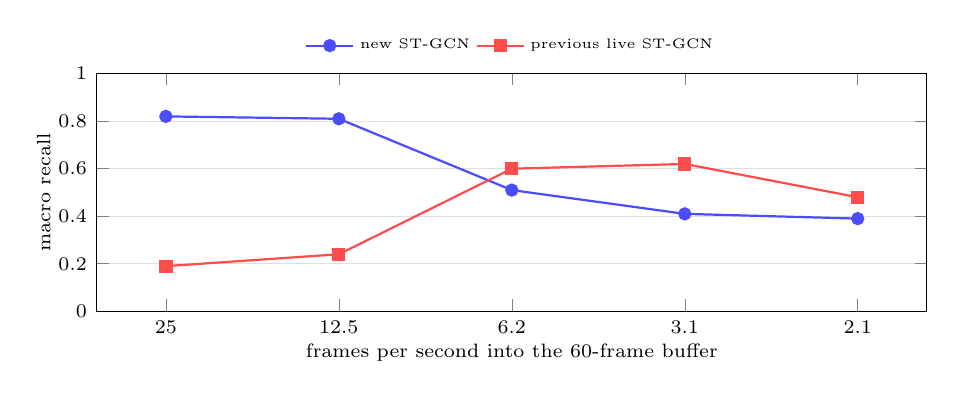
\begin{tikzpicture}
\begin{axis}[width=\linewidth,height=4.6cm,ymin=0,ymax=1,symbolic x coords={25,12.5,6.2,3.1,2.1},xtick=data,x tick label style={font=\scriptsize},y tick label style={font=\scriptsize},
  xlabel={frames per second into the 60-frame buffer},xlabel style={font=\scriptsize,yshift=3pt},ylabel={macro recall},ylabel style={font=\scriptsize,yshift=-4pt},
  legend style={font=\tiny,at={(0.5,1.04)},anchor=south,legend columns=2,draw=none},ymajorgrids,grid style={gray!25},enlarge x limits=0.1]
\addplot[blue!70,mark=*,thick] coordinates {(25,0.82)(12.5,0.81)(6.2,0.51)(3.1,0.41)(2.1,0.39)};
\addplot[red!70,mark=square*,thick] coordinates {(25,0.19)(12.5,0.24)(6.2,0.60)(3.1,0.62)(2.1,0.48)};
\legend{new ST-GCN,previous live ST-GCN}
\end{axis}
\end{tikzpicture}
\caption{ST-GCN input-rate contract}\end{subfigure}
\caption{(a)~Rules-only, \vfour{}, the average of both MLPs, the veto lifted when rules agree, and the cascade. (b)~Per-pose recall and precision of the final ST-GCN on videos it never trained on (dashed: 0.70 bar; warrior~2 and plank have few held-out windows). (c)~Macro recall on held-out videos when the 60-frame buffer is filled at different rates; the new model needs training-rate windows, the previous model was partly trained on slow windows.}
\label{fig:charts}
\end{figure}

\subsection{Baselines: is the neural network necessary?}\label{sec:baselines}
To answer ``compared with what?'' we trained standard methods on exactly the rows the new MLP was trained on (136{,}506 rows of 15 zero-$z$ angles: cue-verified video frames, training photos and photos of other poses labelled transition/unknown) and scored them on the same photos with the same metrics: $k$-NN ($k{=}15$, distance-weighted), an RBF SVM, logistic regression, a 300-tree random forest, and a plain MLP (256--256--128, ReLU, no residual blocks or batch normalisation). The SVM, forest and logistic regression use class-balanced weights; the SVM sees at most 20{,}000 class-balanced rows, the other methods between 64{,}000 and 115{,}000. These runs use one random seed and were executed on Kaggle. Table~\ref{tab:baseline} and Fig.~\ref{fig:baseline} report two held-out sets: the 1{,}685 public photos (same public datasets as the training photos, disjoint files) and the frozen \emph{wild} Commons-103 photos from another source, scored out-of-fold.
\begin{table}[t]
\centering\footnotesize\setlength{\tabcolsep}{3.5pt}
\caption{Standard methods on the same data and held-out photos (bold: best in column). Public: 1{,}685 held-out photos (1{,}037 other poses). Wild: frozen Commons-103, out-of-fold (a different source; with 103 photos, gaps under $\sim$10 points are within noise). $^\dagger$first of two runs.}\label{tab:baseline}
\begin{tabular}{@{}lrrrr@{}}
\toprule
 & \multicolumn{3}{c}{Public held-out} & Wild \\
Method & Overall & False alarm & Poses pass & Overall \\ \midrule
Production before (\vfour{} + rules) & 36.9\% & 78.3\% & 0 & 37.9\% \\
Logistic regression$^\dagger$ & 29.7\% & 95.8\% & 1 & -- \\
$k$-NN & 58.6\% & 55.7\% & 1 & 50.5\% \\
SVM (RBF) & 58.4\% & 56.2\% & 3 & 52.4\% \\
Plain MLP & 80.9\% & 19.1\% & 3 & 47.6\% \\
Random forest & \textbf{85.3\%} & \textbf{9.8\%} & 7 & 35.0\% \\
\vfour{} alone & 42.9\% & 81.5\% & 1 & \textbf{60.2\%} \\
New 3-head model alone & 79.6\% & 22.6\% & 3 & 49.5\% \\
Cascade (ours) & 78.9\% & 20.8\% & 7 & 55.3\% \\ \bottomrule
\end{tabular}
\end{table}
\runin{Findings.} (1)~Linear, nearest-neighbour and kernel models are poor at telling ``another pose'' from ``one of mine'' (false alarms 56--96\%). (2)~A plain MLP matches the residual 3-head model on the public photos (80.9\% against 79.6\%): the residual trunk is not what buys accuracy, and what the 3-head design adds is the form and deviation outputs from one small forward pass. (3)~A random forest is better than the cascade on the public held-out photos: 85.3\% against 78.9\% overall and 9.8\% against 20.8\% false alarms, with seven passing poses each (nine in an earlier run with a different random subsample; the number of poses clearing a fixed bar flips with small changes, so we read little into it).

\begin{figure}[t]
\centering
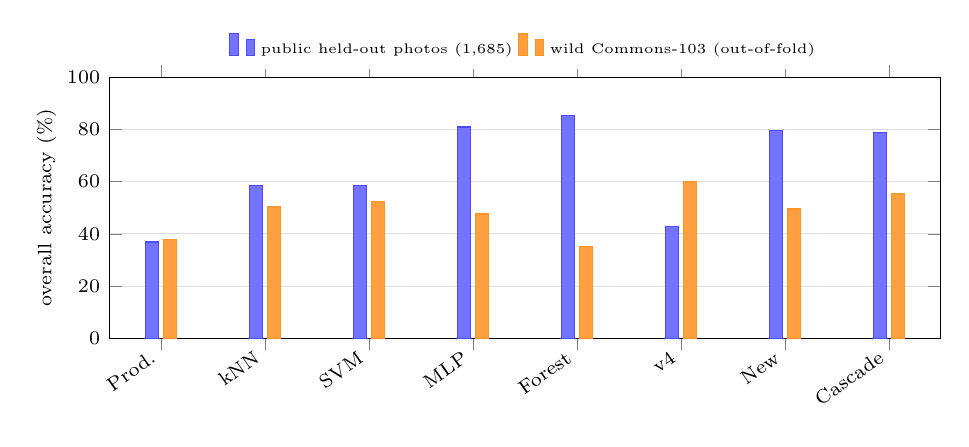
\begin{tikzpicture}
\begin{axis}[ybar,bar width=4.6pt,width=\columnwidth,height=4.9cm,ymin=0,ymax=100,ylabel={overall accuracy (\%)},ylabel style={font=\scriptsize,yshift=-3pt},
  symbolic x coords={Prod.,kNN,SVM,MLP,Forest,v4,New,Cascade},xtick=data,x tick label style={font=\scriptsize,rotate=35,anchor=east},y tick label style={font=\scriptsize},
  legend style={font=\tiny,at={(0.5,1.03)},anchor=south,legend columns=2,draw=none},enlarge x limits=0.07,ymajorgrids,grid style={gray!25}]
\addplot[fill=blue!55,draw=blue!70] coordinates {(Prod.,36.9)(kNN,58.6)(SVM,58.4)(MLP,80.9)(Forest,85.3)(v4,42.9)(New,79.6)(Cascade,78.9)};
\addplot[fill=orange!75,draw=orange!85] coordinates {(Prod.,37.9)(kNN,50.5)(SVM,52.4)(MLP,47.6)(Forest,35.0)(v4,60.2)(New,49.5)(Cascade,55.3)};
\legend{public held-out photos (1{,}685),wild Commons-103 (out-of-fold)}
\end{axis}
\end{tikzpicture}

\caption{The ranking of methods changes with the photo source. Prod.: production before (rules); MLP: plain MLP; New: the new 3-head model alone; Cascade: ours. The forest leads on photos from the training sources and trails every learned method on wild photos.}
\label{fig:baseline}
\end{figure}
\runin{Is the forest's lead a memorisation artefact?} We audited the public test set by the distance of each photo to its nearest training photo in standardised angle space. Exact near-duplicates are rare: only 0.3\% of the 1{,}685 photos lie within 0.05 of a training photo and 4.4\% within 0.2. The forest's lead also holds in every distance quartile, including the farthest (Q4: 84.6\% against 77.0\% for the cascade, Table~\ref{tab:audit}), although every method is most accurate on photos closest to training photos.
\begin{table}[t]
\centering\footnotesize\setlength{\tabcolsep}{3.5pt}
\caption{Public held-out photos split into quartiles of distance to the nearest training photo (Q1 closest; 421--422 photos each): overall accuracy / false-alarm rate.}\label{tab:audit}
\begin{tabular}{@{}lrrrr@{}}
\toprule
Method & Q1 & Q2 & Q3 & Q4 \\ \midrule
Random forest & 93.1 / 16.2 & 82.7 / 19.6 & 81.0 / 9.2 & 84.6 / 1.7 \\
Plain MLP & 91.7 / 14.8 & 78.6 / 28.0 & 75.8 / 21.3 & 77.7 / 13.2 \\
New 3-head model alone & 90.5 / 16.2 & 77.9 / 32.9 & 74.1 / 25.2 & 75.8 / 16.3 \\
Cascade (ours) & 89.1 / 16.2 & 76.2 / 32.0 & 73.4 / 23.2 & 77.0 / 13.5 \\ \bottomrule
\end{tabular}
\end{table}
But the public held-out photos come from the same public datasets as the training photos, and on the wild Commons-103 set the ranking reverses: the forest is the weakest learned method (35.0\%), 13--25 points below the SVM (52.4\%), $k$-NN (50.5\%), plain MLP (47.6\%), the new network (49.5\%), the cascade (55.3\%) and \vfour{} (60.2\%). We read this as: tree ensembles are the strongest method on photos like the training photos and the weakest on photos from another source, so no method is best on both. The cascade is within seven points of the best method on each set and keeps false alarms at 20.8\%; a tree--network ensemble is the obvious next experiment (Section~\ref{sec:limits}). We keep the 3-head network because the form and deviation heads, the 0.36\,M-parameter footprint and the better behaviour on wild photos matter for a coach that must run on any phone, and because it is the architecture of the project proposal; we do not claim it is the best frame-level namer on same-source photos.

\subsection{Held-out videos: the ST-GCN}
On three folds split by video (24 videos, 8{,}002 windows, 60 frames, stride 12), the final target-pose ST-GCN reaches 82.2\% overall; because 60\% of the windows are transition/unknown this flatters it, so we also report 78.0\% macro recall over the nine classes (76.9\% over the eight poses). Three poses clear the bar: child's pose (recall/precision $.74/.91$), corpse ($1.00/.85$) and downward dog ($.83/.77$); seated easy, tree and triangle are within about 0.07 of it (Fig.~\ref{fig:charts}b). The model is conservative: its misses go to transition/unknown instead of to another pose. Warrior~II and plank fail on precision ($.26$, $.18$): 158 transition windows are called Warrior~II and plank has only 30 windows. A less conservative threshold chosen without leakage (an offset on the transition logit, picked on two folds and applied to the third) leaves overall accuracy at 81.9\% and raises the passing poses to four (child, downward dog, triangle, seated easy; corpse then drops below the precision bar); no offset reaches six. We therefore claim three poses (four with the cross-fitted threshold) for the ST-GCN and keep the ``seven poses'' claim for the frame cascade.

\runin{Old versus new.} Table~\ref{tab:stgcn} scores the sequence model that was live until this work against the new one on the same held-out windows. The 12 videos that arrived after the old models were trained make that subset clean for them. The old live model had macro recall of 18.8\% and answered (with confidence $\ge$ its gate) on 2.8\% of true-pose windows; the new model answers on 50.5\% at 88.1\% precision. The old model's named transitions are not measured here and the new model has a single generic transition class.
\begin{table}[t]
\centering\footnotesize
\caption{ST-GCN versions on the same held-out windows (12 videos new to the old models; bold: best in column). ``Answered'' is the share of true-pose windows that reach the UI, with its precision.}\label{tab:stgcn}
\begin{tabular}{@{}lrrrr@{}}
\toprule
Model & Overall & Macro rec. & Passing & Answered / prec. \\ \midrule
Old original (Jul) & 67.3\% & 11.6\% & 0 & 0\% / -- \\
Old v2 & 67.8\% & 13.2\% & 0 & 1.8\% / 100\% \\
Old live & 68.9\% & 18.8\% & 0 & 2.8\% / 93.8\% \\
New & \textbf{76.9\%} & \textbf{82.1\%} & 2 & \textbf{50.5\% / 88.1\%} \\ \bottomrule
\end{tabular}
\end{table}

\runin{The input-rate contract.} Fig.~\ref{fig:charts}c re-scores the same videos while subsampling every $k$-th frame. The new model keeps macro recall $0.82$ at the training rate (25\,fps) and $0.81$ at 12.5\,fps, then loses it ($0.51$ at 6.2\,fps, $0.41$ at 3.1\,fps, $0.39$ at 2.1\,fps); the old model, partly trained on slow windows, is better at slow rates but never exceeds $0.62$. This is why the web app now fills a time-based 25\,fps buffer. A server audit found the backend architecture and normalisation identical to the trainer's (maximum logit difference 0.0 on 64 windows) and the deployed endpoint matching a local run of the same weights on 40/40 and 60/60 windows, so the weakness of the old model was generalisation, not serving.
\runin{Sequence baselines (GPU run, Kaggle T4, 1915\,s).} Six sequence models were trained under one recipe (AdamW, cosine schedule, class-weighted loss, 10 epochs, at most 6{,}000 windows per class, last epoch scored, one seed) and scored on the same three video folds. Results (overall / macro recall over nine classes / over eight poses / poses passing): LSTM 83.0\% / 89.5\% / 91.0\% / 4; BiLSTM with attention 87.1\% / 89.6\% / 90.1\% / 5; temporal CNN 81.5\% / 89.7\% / 91.4\% / 4; MLP on window mean and standard deviation (86\,k parameters) 85.3\% / 94.4\% / 96.4\% / 5; ST-GCN without the skeleton graph 77.1\% / 84.8\% / 86.4\% / 4; ST-GCN 76.0\% / 86.4\% / 88.6\% / 4. The skeleton graph helps only slightly over the graph-free variant, and simpler models match or exceed the ST-GCN; an ST-GCN fold trains in about 290\,s against 6--15\,s for the others. Raw results: \texttt{planning/kaggle\_transfer/kernel\_baselines\_seq\_gpu\_arko/results\_seq\_gpu\_v1.json}.

\subsection{Does the form score mean anything?}
No labelled good-versus-bad-form data exist for these poses, so we use a property test: on 648 held-out in-vocabulary photos, five trials each, one joint is broken by $45^\circ$. Table~\ref{tab:form} shows that the new gate's form score is high on good form (0.81) and drops in 85.0\% of trials, the best of the four models, while the deviation head's top-ranked joint is the broken one in only 12.4\% of trials (chance 6.7\%), which is why per-joint cues come from the angle bands.
\begin{table}[t]
\centering\footnotesize
\caption{Property test: one joint broken by $45^\circ$ (chance for ``points at the broken joint'' is 6.7\%; bold: best in column).}\label{tab:form}
\begin{tabular}{@{}lrrr@{}}
\toprule
Model & Score, good form & Score drops & Top joint correct \\ \midrule
19 Jul original & 0.28 & 65.0\% & 8.1\% \\
3 Sep retrain & 0.67 & 74.9\% & \textbf{18.2\%} \\
21 Sep \vfour{} & 0.79 & 59.2\% & 6.7\% \\
New & \textbf{0.81} & \textbf{85.0\%} & 12.4\% \\ \bottomrule
\end{tabular}
\end{table}
The same test on the deployed endpoint with real MediaPipe angles from eight instructor clips gives a mean score of 0.94 while held, 0.25 with the left knee broken (a drop on every probe of every clip) but 0.92 with the left elbow broken: the score collapses for leg errors and is nearly blind to arm errors. Arm errors can only be caught, if at all, by the angle-band layer, and we do not claim whole-body form checking. (These clips are in the gate's training data, so this is a regression check of the deployed path, not a generalisation number.)

\subsection{End-to-end checks on a real phone and on recorded video}
\runin{On-phone photo test.} With the production app running on the POCO M7 Pro through its CPU engine and a Wikimedia photo standing in for the camera, every answer of the live server was logged (Table~\ref{tab:phone}); a photo counts if the most frequent of three answers is the expected pose, and a pose passes at $\ge50\%$ of its photos. Eight of eleven poses pass; of the seven poses that passed the held-out benchmark, the six tested here all pass, while mountain, cobra and child's pose do not (mountain and cobra were already weak). These are still photos with labels taken from file titles, and the models trained on Commons photos, so some may have been seen: the test checks the on-phone path (engine, landmarks, server, label), not generalisation.
\begin{table}[t]
\centering\footnotesize
\caption{On-phone photo test (photos correct / tested; a pose passes at 50\% or more). Two photos had no person found.}\label{tab:phone}
\begin{tabular}{@{}lcc@{\hspace{10pt}}lcc@{}}
\toprule
Pose & Correct & & Pose & Correct & \\ \midrule
Tree & 6/6 & pass & Chair & 3/5 & pass \\
Triangle & 5/5 & pass & Corpse & 2/4 & pass \\
Warrior II & 3/3 & pass & Child's pose & 1/3 & miss \\
Downward dog & 4/4 & pass & Cobra & 1/5 & miss \\
Seated easy & 4/5 & pass & Mountain & 0/5 & miss \\
Plank & 3/4 & pass & & & \\ \bottomrule
\end{tabular}
\end{table}

\runin{Live replay on recorded video.} We replayed eight clips of held poses (six poses, real MediaPipe on instructor video) against the deployed Space as the app would call it: seven of eight clips scored $\ge0.81$ frame-level accuracy while the pose was held (call-weighted 88.4\%), with zero failed API calls. One Seated-easy clip failed (0.06: named upward dog throughout), so Seated easy is not reliable live. On three clips of continuous movement the system reported ``transitioning'' for 74\%, 92\% and 79\% of frames. All eight clips come from videos in the training data of the gate, so this is a plumbing check; the ST-GCN, deployed after, answered correctly on 100\% of calls for the four poses it knows and stayed ``transition/unknown'' for mountain and lunge, which are outside its vocabulary.

\subsection{The interface}
Fig.~\ref{fig:ui} shows the deployed interface on the phone in the three languages and both themes, in free and guided mode, and the public landing page. The skeleton overlay uses the colours of Section~\ref{sec:models} and the score ring, ``For your body'' personal score and coaching cue update about every 1.5\,s.
\begin{figure}[t]
\centering
\begin{subfigure}[t]{0.165\textwidth}\centering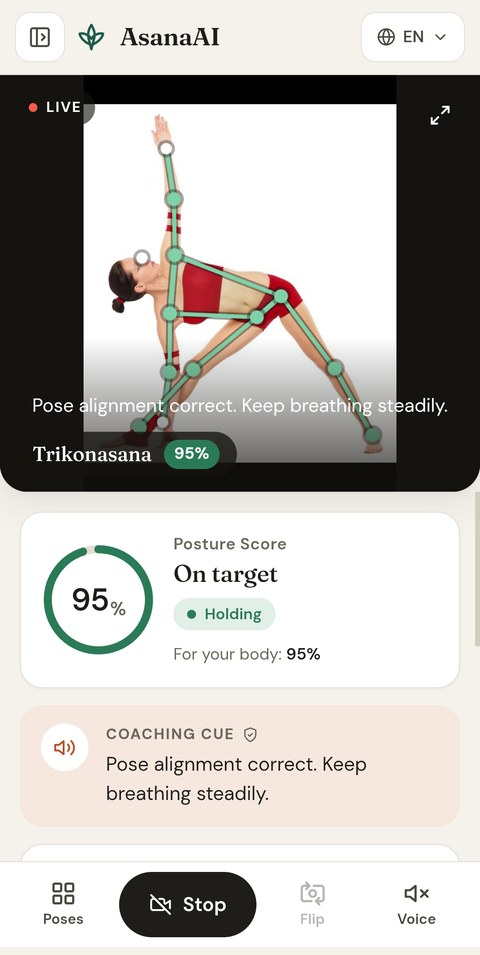
\includegraphics[width=\linewidth]{figures/ui_triangle_en.jpg}\caption{Free mode, English, light}\end{subfigure}\hfill
\begin{subfigure}[t]{0.165\textwidth}\centering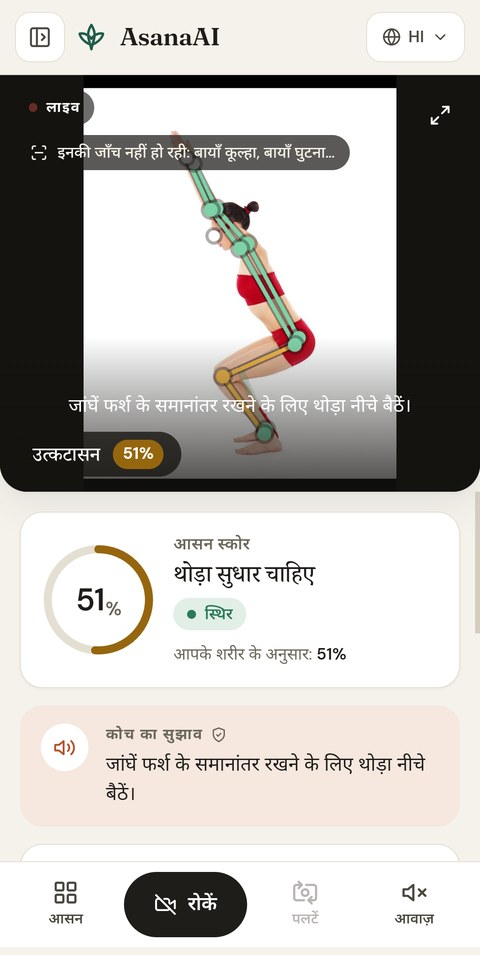
\includegraphics[width=\linewidth]{figures/ui_chair_hi.jpg}\caption{Hindi: 51\% form, amber}\end{subfigure}\hfill
\begin{subfigure}[t]{0.165\textwidth}\centering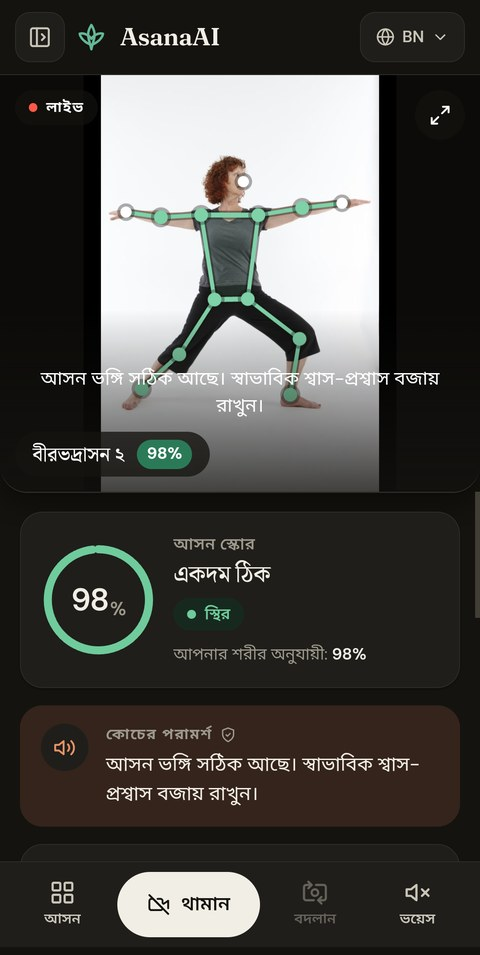
\includegraphics[width=\linewidth]{figures/ui_warrior_bn_dark.jpg}\caption{Bengali, dark theme}\end{subfigure}\hfill
\begin{subfigure}[t]{0.165\textwidth}\centering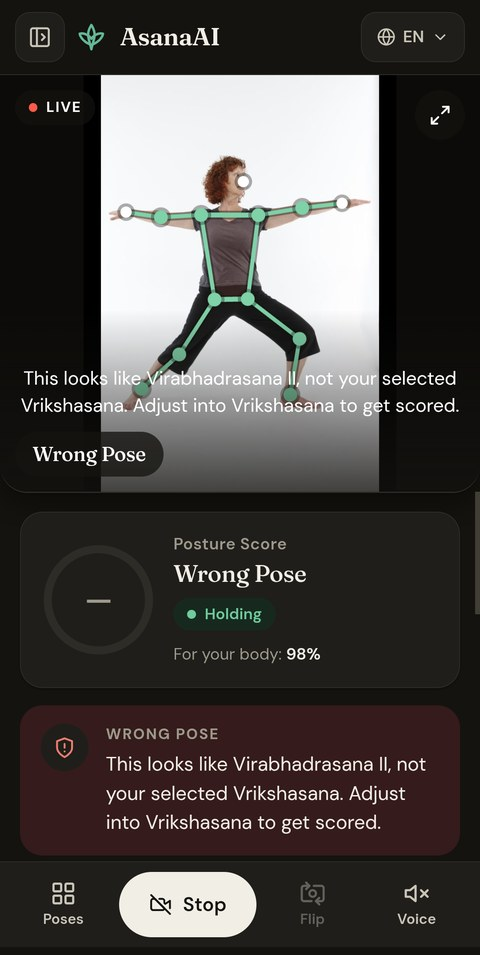
\includegraphics[width=\linewidth]{figures/ui_guided_wrong.jpg}\caption{Guided: wrong-pose card}\end{subfigure}\hfill
\begin{subfigure}[t]{0.165\textwidth}\centering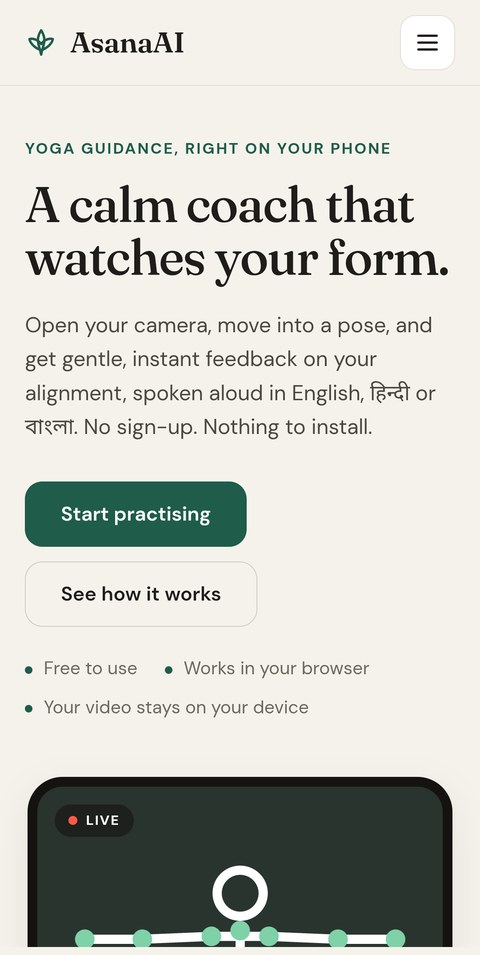
\includegraphics[width=\linewidth]{figures/landing_light.jpg}\caption{The public landing page}\end{subfigure}
\caption{The deployed interface on a POCO M7 Pro, a credited Wikimedia photo standing in for the camera (no live person): (a)~Trikonasana, 95\%; (b)~Utkatasana with the Hindi cue, 51\% in amber and a chip naming the joints not checked; (c)~Virabhadrasana~II in Bengali; (d)~guided mode with Vrikshasana selected while a Warrior~II photo is shown: the score is withheld and the app names the pose it sees; (e)~the public landing page (light theme). Photos by Kennguru (a, b; CC BY 3.0) and lululemon athletica (c, d; CC BY 2.0), via Wikimedia Commons.}
\label{fig:ui}
\end{figure}

\section{Comparison with Related Work}\label{sec:compare}
Direct numeric comparison with other groups is not possible (we could not obtain their systems; datasets, vocabularies and splits differ), so Table~\ref{tab:related} compares what each work reports, using only what the cited sources state; ``n/r'' means not reported in the sources we read, not that the feature is absent.
\begin{table}[t]
\centering\scriptsize
\caption{What each work reports (qualitative; n/r = not reported in the sources we read).}\label{tab:related}
\begin{tabularx}{\textwidth}{@{}p{2.2cm}p{3.1cm}p{3.6cm}XXX@{}}
\toprule
Work & Task and input & Evaluation as described & Hidden joints & Feedback to the user & Runs on a phone / image stays local \\ \midrule
Chen et al.\ \cite{chen2014yoga} & posture recognition from silhouette star skeleton & n/r & n/r & links to training information & n/r \\
Yoga-82 \cite{verma2020yoga82} & image classification, 82 poses, 3-level labels & dataset benchmark of CNNs; motivates occlusion and viewpoint variety & dataset difficulty only & none (classification) & n/r \\
Thoutam et al.\ \cite{thoutam2022yoga} & incorrect posture in uploaded videos & n/r & n/r & abnormal angles and advice & uploaded video; n/r \\
Mohiuddin et al.\ \cite{mohiuddin2025skeleton} & Yoga-16 (1{,}280 images, 16 poses); MediaPipe / YOLOv8 skeletons vs.\ images & 96.09\% on a 256-image test split of a dataset split into 896/128/256 & none & none & n/r \\
PosePilot \cite{gadhvi2025posepilot} & LSTM, BiLSTM + attention on video; new video dataset & evaluation detail n/r in the abstract & not discussed & instant corrective feedback & edge devices (design goal); n/r \\
Pose-to-Pose \cite{dittakavi2025pose2pose} & generating target poses (transitions), counterfactuals & new benchmark (PoseHPT) & n/r & not a coach & n/r \\
Liao et al.\ \cite{liao2020rehab} & scoring rehabilitation exercise quality & n/r here & n/r & quality score & n/r \\ \midrule
AsanaAI (this work) & landmark angles + 60-frame skeleton windows; cascade + ST-GCN & held-out photos and held-out videos only; false-alarm metric; controlled baselines & abstains on hidden joints; CLIFF vs.\ mirror measured & per-joint cues, three languages, screened, escalating & \cmark\ tested on a budget phone / \cmark\ only numbers leave the device \\ \bottomrule
\end{tabularx}
\end{table}

\runin{What we add.} To the best of our reading, the works above do not report (i)~a false-alarm rate on photos of poses outside the vocabulary, which is what matters when a user is in a pose the app does not know; (ii)~a split by video or by held-out source, as opposed to a split of a single image set (Yoga-16's test split is 256 images from the same 1{,}280); (iii)~how hidden joints are handled, or an experiment comparing recovery methods; (iv)~a deployment through a GPU driver that fails; or (v)~privacy by construction, multilingual coaching with a safety screen and an offline mode with a parity proof. We also show, on our own models, how large the random-split illusion can be: the first MLP reported 91.5\% validation accuracy and scored 26.8\% on Commons photos it had never seen, and the first ST-GCN reported 82.6\% validation accuracy but only 11.6\% macro recall on held-out videos.

\runin{Where others are stronger, and what we do not do.} Yoga-82 covers 82 poses with a hierarchy and thousands of images, while our guided mode covers eight poses and only three or four pass on video; PosePilot's temporal feedback is delivered at every stage of a movement, whereas ours is per-frame cues plus a flow check; Pose-to-Pose generates how to move between poses and we do not; Liao et al.\ learn a quality score whereas our form score is not validated against human labels. Accuracies such as Yoga-16's 96.09\% come from a different protocol and are not comparable to ours; the controlled comparison is the one against standard methods on our own data and held-out sets (Section~\ref{sec:results}).

\section{Limitations and Future Work}\label{sec:limits}
\runin{Lessons.} (1)~A random split measures memory; only held-out numbers are evidence \cite{kapoor2023leakage}. (2)~Train/serve skew hides in plain sight: raw-$z$ training angles versus served zero-$z$ angles ($14^\circ$ median gap), and a sequence model fed at 0.5\,fps that was trained at 25\,fps, both of which looked like ``model problems'' \cite{sculley2015debt}. (3)~Silent fallbacks are the dangerous kind: a retired language-model name returned the safe template for every request and looked like success, and a phone with a faulty GPU path crashed inside a driver instead of ``having no WebGL''. (4)~No method wins on every photo source, so report more than one held-out set.

\runin{Limitations.}
\begin{itemize}
\item \emph{No live-person accuracy yet.} All end-to-end tests use photos or recorded video; the one live test with a person had nobody in view. A study with practitioners and instructors is needed.
\item \emph{The form score is not validated against human judgement.} It is checked only by a perturbation test, it is nearly blind to arm errors (0.94$\to$0.92 when an elbow is broken), and the learned deviation head is close to chance (12.4\% vs.\ 6.7\%); joint-level cues rest on hand-set angle bands.
\item \emph{Tree and Lunge have no angle bands,} so the app gives no per-joint feedback for them (neutral limbs; before 2026-10-07 the near-chance learned head's guesses were drawn, Fig.~\ref{fig:occ}d). Tree is one of the eight guided poses; hand-set bands with an either-leg rule are the obvious next step.
\item \emph{Weak poses.} Mountain, cobra and child's pose fail on the phone photo test; chair and corpse pass at only 50--60\%; Seated easy failed on one live clip (named upward dog throughout); the ST-GCN reliably handles three poses.
\item \emph{Small data.} 24 videos and public photo sets; some per-pose test sets have fewer than 30 items; single-seed baselines; the held-out public photos share their sources with the training photos (exact near-duplicates are rare, Table~\ref{tab:audit}, but the ranking of methods changes on wild photos, Table~\ref{tab:baseline}); the wild set has only 103 photos.
\item \emph{The skeleton graph is not shown to be necessary.} Under one recipe, simpler sequence models match or exceed the ST-GCN at held-pose recognition (Section~\ref{sec:results}).
\item \emph{Occlusion.} We abstain rather than recover; the pose name can still be influenced by a hallucinated hidden joint; the CLIFF study is small (141 cases, one asymmetric pose, a synthetic box, MediaPipe as reference).
\item \emph{Personalisation.} The range-of-motion profile is not user-tested and a profile learned from a poor stance could forgive real errors; the demonstration profile came from a still photo.
\item \emph{Languages.} The Hindi and Bengali interface text and cue templates were checked by a native speaker of both languages on the team; they have not had an independent review by yoga instructors or users, the language-model paraphrases are generated at run time and are not reviewed, and the forbidden-word screen is a list of English words, so it cannot flag unsafe wording in a Hindi or Bengali paraphrase; those languages rely on the reviewed templates and the escalation back-off.
\item \emph{Hardware.} Verified on one phone model and desktop browsers; other phones with the same GPU, other browsers, battery and thermal behaviour were not measured. The free-tier server can sleep, in which case basic mode applies (rules only: 36.9\% accuracy and 78.3\% false alarms on held-out photos).
\item \emph{Not a medical device.} We make no claim about injury prevention; no outcome study exists.
\end{itemize}

\runin{Future work.} (i)~A live user study in which instructors rate form, producing the labelled good/bad-form data the form head lacks; (ii)~retraining the form and deviation heads with arm perturbations and with those labels; (iii)~a tree--network ensemble for naming, since a random forest is the strongest method on same-source photos and the weakest on wild ones, so the two may be complementary (untested); (iv)~viewpoint-robust features (3-D lifting) and a larger pose vocabulary; (v)~opt-in server-side mesh recovery for hidden joints with explicit image consent, now that its benefit for legs and asymmetric poses is measured; (vi)~independent review of the Hindi and Bengali coaching by instructors, and language-specific safety screens; (vii)~flow scores and named transitions, the tasks on which a temporal model must prove its value over static statistics; (viii)~more devices, including battery and thermal tests.

\section{Conclusion}
AsanaAI shows that a yoga coach can run in a browser, keep the camera image on the device and still work on a budget phone, provided evidence is held to a strict standard. Evaluated only on data never trained on, a gated cascade of residual MLPs names poses on 78.9\% of held-out photos with 20.8\% false alarms and seven passing poses, an ST-GCN with the right input rate reaches 78.0\% macro recall on held-out videos, controlled baselines show that no frame-level method wins on every photo source, and the system degrades gracefully: it abstains on hidden joints, falls back through three pose engines, and keeps coaching offline. We also report what it cannot do yet, which is as important to a person who might follow its advice.

\runin{Availability.} App: \url{https://yoga-posture-correction-system.vercel.app} (landing page /landing); API: \url{https://arko007-yoga-pose.hf.space}; code: \url{https://github.com/Anamitra-Sarkar/yoga-posture-correction-system}; training data and code: Hugging Face dataset Arko007/Yoga-1M (the transcripts are withheld because they are copyrighted speech).

\section{Verification, Audit and Fixes}\label{sec:audit}
This section records what was checked before the project was written up, what was found, and what was changed. The full evidence is in \texttt{docs/REPO\_AUDIT\_2026-10-07.md}; none of this belongs in the research paper.

\subsection{Method}
All checks were read-only or black-box: tracked files, documentation, code, CI runs and deployments were inspected, and the deployed backend was queried over HTTP. Nothing was built or trained on the development machine (3.7\,GB RAM). A live smoke test (\texttt{backup/verify\_live.sh}) now makes seven assertions against production.

\subsection{Findings that affect users or safety}
\begin{table}[h]
\centering\footnotesize
\begin{tabularx}{\textwidth}{@{}p{0.7cm}Xp{4.2cm}@{}}
\toprule
\# & Finding & Status \\ \midrule
A1 & Tree and Lunge have no angle bands. With the cascade on, their per-joint deviations came from the learned deviation head, which is close to chance, so a correct Tree could show a coral standing leg and a cue could name the wrong joint. Evidence: a hand-built Tree frame returned deviations of 72--73$^\circ$ on a straight leg; screenshot in the repository. & \textbf{Fixed and live.} The cascade now returns zero deviations (\texttt{none\_no\_bands}); the web app draws neutral limbs (\texttt{NO\_BAND\_POSES}); verified against production and in the shipped JavaScript. \\
A2 & The unsafe-word screen was a list of English words, while the language-model paraphrase is live in Hindi and Bengali. & Draft word lists with a regression test on branch \texttt{fix/safety-screen-hi-bn}; awaiting the native-speaker review (review sheet in \texttt{docs/}). Not shipped. \\
A3 & Code defaults were the old behaviour (cascade off, old ST-GCN); production was correct only because of Space variables. & \textbf{Fixed and live.} Defaults now equal the benchmarked configuration; the variables remain for rollback. \\
A4 & Body orientation is computed and sent but ignored while the cascade is on. & Documented. \\
A5 & The personal profile works as designed but is unvalidated; a profile spanning $0^\circ$--$180^\circ$ forgives every deviation. & Documented; user study is future work. \\ \bottomrule
\end{tabularx}
\end{table}

\subsection{Hygiene findings}
The live smoke test pre-dated the cascade, so two of its checks passed while testing nothing; it was rewritten with realistic frames and assertions. The README overstated the safety filter and listed orientation as a pipeline input (corrected). 15 merged remote branches, each building a preview deployment, were deleted after each was verified as an ancestor of \texttt{main}; one unmerged branch was left for the owner. Other items, not changed: ``Digital Twin'' remains the internal name in some comments and types while the interface says ``Your range of motion''; a June integration script sits outside the tests directory; a manifest shortcut opens an unused query parameter; CI does not run the backend tests; about 17\,MB of old checkpoints are tracked in git; the Expo companion still carries template scaffolding and the older six-pose vocabulary.

\subsection{Verified without findings}
No secrets or tokens in any tracked file; 114 translation keys in each of English, Hindi and Bengali with none missing or untranslated (checked by a native speaker); all relative documentation links resolve; CI green; the Vercel production deployment equals \texttt{main}; all seven model files exist on the model repository; the owner's saved app settings were restored after every automated screenshot run.

\subsection{Calibration check}
The calibration feature was exercised end to end on the deployed server (Section~\ref{sec:calib}): a profile containing a deviating joint's angle raises the personal score, a profile that does not leaves it unchanged, and the universal score never changes. The check is repeatable with the smoke test.

\subsection{A measurement worth recording}
End-to-end request latency from a residential connection in India was 0.97\,s at the median (p95 1.27\,s, 32 requests) although server compute is 7--9\,ms: the delay is the network to the hosting region. This motivates running the small MLPs on the device.

\section{Repository, Operations and Reproducibility}\label{sec:repo}
\subsection{Layout}
\begin{tabularx}{\textwidth}{@{}lX@{}}
\toprule
Path & Contents \\ \midrule
\texttt{backend/} & FastAPI service (also the Hugging Face Space): models, rule engine, cascade, coaching, tests, tools \\
\texttt{frontend/} & Next.js progressive web app (app at \texttt{/}, website at \texttt{/landing}) and the Capacitor Android project \\
\texttt{mobile/} & separate Expo client \\
\texttt{modal/}, \texttt{planning/} & data and training pipeline, experiments and the Kaggle kernels (including the baseline kernels) \\
\texttt{docs/} & benchmarks, cascade and sequence-model notes, training lessons, live-test clips, the audit \\
\texttt{paper/} & the research paper (conference format) \\
\texttt{report/} & this report \\
\texttt{backup/} & resume notes, dated copies of key documents, the live smoke test, phone-debugging tools \\ \bottomrule
\end{tabularx}

\subsection{Deployment and operations}
Pushing to \texttt{main} with changes under \texttt{backend/} or to \texttt{README.md} synchronises the Hugging Face Space (GitHub Actions); Vercel builds \texttt{main} for production and every other branch as a preview. Since 2026-10-07 the backend defaults equal the benchmarked configuration (pose cascade on, \texttt{stgcn\_target\_v1}); rollback uses the Space variables \texttt{ENABLE\_POSE\_CASCADE=0} and \texttt{STGCN\_MODEL\_FILE}/\texttt{STGCN\_ENCODER\_FILE} set to the previous files. The optional paraphrase needs a language-model API key stored as a Space secret. The free-tier Space sleeps when idle, in which case the browser answers in basic mode.

\subsection{Testing}
The backend has 70 test functions in nine files (stub models, no network); the two files touched by the 2026-10-07 changes pass (21 tests) and the safety-screen draft adds 36. The live smoke test checks the deployed system after every backend deployment. The Android workflow also type-checks the Expo companion.

\subsection{Compute policy}
Training and baselines run on Kaggle (CPU or GPU kernels) or Codespaces, never on the development machine; Hugging Face model files are never overwritten (new names only); \texttt{kaggle kernels output} is avoided and logs are read through the kernel's REST log field. The sequence-model baselines (LSTM, BiLSTM with attention, temporal CNN, window-statistics MLP, ST-GCN with and without the skeleton graph) are in \texttt{planning/kaggle\_transfer/kernel\_baselines\_seq*}.

\subsection{Rebuilding the documents}
\texttt{cd paper \&\& python3 make\_refs.py \&\& pdflatex asanaai\_research\_paper.tex} (twice) and likewise in \texttt{report/}. IEEEtran's bibliography style is not installed on the development machine, so \texttt{make\_refs.py} builds the numbered reference list from the verified \texttt{references.bib}.


% generated by make_refs.py from references.bib -- do not edit by hand
\begin{thebibliography}{25}
\bibitem{unga2014yoga} United Nations General Assembly, ``Resolution A/RES/69/131: International Day of Yoga,'' adopted 11 December 2014.
\bibitem{cramer2013yoga} H. Cramer, R. Krucoff, and G. Dobos, ``Adverse Events Associated with Yoga: A Systematic Review of Published Case Reports and Case Series,'' \textit{PLoS ONE}, vol.~8, no.~10, 2013, Art. no.~e75515.
\bibitem{bazarevsky2020blazepose} V. Bazarevsky, I. Grishchenko, K. Raveendran, T. Zhu, F. Zhang, and M. Grundmann, ``BlazePose: On-device Real-time Body Pose Tracking,'' arXiv:2006.10204, 2020.
\bibitem{lugaresi2019mediapipe} C. Lugaresi \textit{et al.}, ``MediaPipe: A Framework for Building Perception Pipelines,'' arXiv:1906.08172, 2019.
\bibitem{kapoor2023leakage} S. Kapoor and A. Narayanan, ``Leakage and the Reproducibility Crisis in Machine-Learning-Based Science,'' \textit{Patterns}, vol.~4, no.~9, 2023, Art. no.~100804.
\bibitem{radford2023whisper} A. Radford, J. W. Kim, T. Xu, G. Brockman, C. McLeavey, and I. Sutskever, ``Robust Speech Recognition via Large-Scale Weak Supervision,'' in \textit{Proc. 40th Int. Conf. Machine Learning (ICML)}, PMLR, vol.~202, 2023, pp.~28492--28518.
\bibitem{yan2018stgcn} S. Yan, Y. Xiong, and D. Lin, ``Spatial Temporal Graph Convolutional Networks for Skeleton-Based Action Recognition,'' in \textit{Proc. AAAI Conf. Artificial Intelligence}, vol.~32, no.~1, 2018, pp.~7444--7452, doi: 10.1609/aaai.v32i1.12328.
\bibitem{li2022cliff} Z. Li, J. Liu, Z. Zhang, S. Xu, and Y. Yan, ``CLIFF: Carrying Location Information in Full Frames into Human Pose and Shape Estimation,'' in \textit{European Conf. Computer Vision (ECCV)}, 2022, doi: 10.1007/978-3-031-20065-6\_34.
\bibitem{chen2014yoga} H.-T. Chen, Y.-Z. He, C.-C. Hsu, C.-L. Chou, S.-Y. Lee, and B.-S. P. Lin, ``Yoga Posture Recognition for Self-training,'' in \textit{MultiMedia Modeling (MMM)}, 2014, pp.~496--505.
\bibitem{verma2020yoga82} M. Verma, S. Kumawat, Y. Nakashima, and S. Raman, ``Yoga-82: A New Dataset for Fine-grained Classification of Human Poses,'' in \textit{Proc. IEEE/CVF Conf. Computer Vision and Pattern Recognition Workshops (CVPRW)}, 2020, pp.~1038--1039.
\bibitem{mohiuddin2025skeleton} M. Mohiuddin, S. M. M. Hossain, S. Khanam, P. Barua, A. Barua, and M. T. Hossain, ``Integrating Skeleton Based Representations for Robust Yoga Pose Classification Using Deep Learning Models,'' arXiv:2512.00572, 2025.
\bibitem{thoutam2022yoga} A. Thoutam \textit{et al.}, ``Yoga Pose Estimation and Feedback Generation Using Deep Learning,'' \textit{Computational Intelligence and Neuroscience}, 2022, doi: 10.1155/2022/4311350.
\bibitem{gadhvi2025posepilot} R. Gadhvi, P. Desai, and Siddharth, ``PosePilot: An Edge-AI Solution for Posture Correction in Physical Exercises,'' in \textit{Iberian Conf. Pattern Recognition and Image Analysis (IbPRIA)}, 2025, arXiv:2505.19186.
\bibitem{dittakavi2025pose2pose} B. Dittakavi, S. Maheshwari, and V. N. Balasubramanian, ``Pose-to-Pose: A New Task and Benchmark for Human Pose Transition in Yoga,'' in \textit{Proc. IEEE/CVF Conf. Computer Vision and Pattern Recognition Workshops (CVPRW)}, 2025, pp.~6138--6147.
\bibitem{liao2020rehab} Y. Liao, A. Vakanski, and M. Xian, ``A Deep Learning Framework for Assessing Physical Rehabilitation Exercises,'' \textit{IEEE Trans. Neural Syst. Rehabil. Eng.}, vol.~28, no.~2, 2020, pp.~468--477, doi: 10.1109/TNSRE.2020.2966249.
\bibitem{cao2021openpose} Z. Cao, G. Hidalgo, T. Simon, S.-E. Wei, and Y. Sheikh, ``OpenPose: Realtime Multi-Person 2D Pose Estimation Using Part Affinity Fields,'' \textit{IEEE Trans. Pattern Anal. Mach. Intell.}, vol.~43, no.~1, 2021, pp.~172--186.
\bibitem{sun2019hrnet} K. Sun, B. Xiao, D. Liu, and J. Wang, ``Deep High-Resolution Representation Learning for Human Pose Estimation,'' in \textit{Proc. IEEE/CVF Conf. Computer Vision and Pattern Recognition (CVPR)}, 2019.
\bibitem{xu2022vitpose} Y. Xu, J. Zhang, Q. Zhang, and D. Tao, ``ViTPose: Simple Vision Transformer Baselines for Human Pose Estimation,'' in \textit{Advances in Neural Information Processing Systems (NeurIPS)}, 2022.
\bibitem{smilkov2019tfjs} D. Smilkov \textit{et al.}, ``TensorFlow.js: Machine Learning for the Web and Beyond,'' arXiv:1901.05350, 2019.
\bibitem{loper2015smpl} M. Loper, N. Mahmood, J. Romero, G. Pons-Moll, and M. J. Black, ``SMPL: A Skinned Multi-Person Linear Model,'' \textit{ACM Trans. Graphics}, vol.~34, no.~6, 2015, pp.~248:1--248:16, doi: 10.1145/2816795.2818013.
\bibitem{geifman2017selective} Y. Geifman and R. El-Yaniv, ``Selective Classification for Deep Neural Networks,'' in \textit{Advances in Neural Information Processing Systems (NeurIPS)}, 2017.
\bibitem{sculley2015debt} D. Sculley \textit{et al.}, ``Hidden Technical Debt in Machine Learning Systems,'' in \textit{Advances in Neural Information Processing Systems (NIPS)}, 2015, pp.~2503--2511.
\bibitem{ioffe2015bn} S. Ioffe and C. Szegedy, ``Batch Normalization: Accelerating Deep Network Training by Reducing Internal Covariate Shift,'' in \textit{Proc. 32nd Int. Conf. Machine Learning (ICML)}, 2015.
\bibitem{hendrycks2016gelu} D. Hendrycks and K. Gimpel, ``Gaussian Error Linear Units (GELUs),'' arXiv:1606.08415, 2016.
\bibitem{he2016resnet} K. He, X. Zhang, S. Ren, and J. Sun, ``Deep Residual Learning for Image Recognition,'' in \textit{Proc. IEEE Conf. Computer Vision and Pattern Recognition (CVPR)}, 2016.
\end{thebibliography}


\end{document}
